%===============================================================================
\chapter{Controle baseado em dados}
\label{chapter:vfrt}
%===============================================================================

%\TODO:: REVER ESTE PARAGRAFO:
%
%Em aplica��es pr�ticas, a descri��o matem�tica da planta n�o � dispon�vel e o sistema deve ser identificado
%baseado nas medidas obtidas deste sistema. Este assunto tem atra�do a aten��o de diversos engenheiros de
%controle desde 1940 com o pioneiro trabalho de Ziegler e Nichols (1942) com ajuste de controladores PID
%industriais. Depois do trabalho de Ziegler e Nichols diversos trabalhos surgiram, muitos em formas de
%aperfei�oamento e extens�es das t�cnicas j� apresentadas, e algumas com desenvolvimentos em novas dire��es
%(\cite{mcmillan1983tuning}, \cite{Haalman1965}). A caracter�stica principal destes m�todos � que eles podem
%ser facilmente utilizados: simples experimentos sobre a planta s�o executados e simples regras 
%s�o aplicadas sobre os dados obtidos. O m�todo VRFT que ser� abordado aqui tem algumas destas 
%caracter�sticas, pois s� requer que apenas um experimento seja executado sobre a planta. 
%\cite{campi_leccini_savaresi2002}

%===============================================================================
%===============================================================================
\section{Defini��es}
\label{sec:vrft_control_data_based}
%===============================================================================
O projeto de controladores baseados em dados consiste em obter, ou estimar, os par�metros de uma fam�lia ou conjunto de 
modelos baseados nos dados obtidos da planta sob an�lise. Os dados utilizados para esta tarefa s�o usualmente os sinais
de entrada e sa�da do sistema.

Como j� foi discutido na se��o (\ref{sec:si_project_experiments}) estes dados podem ser obtidos de
diversas formas. Algumas vezes estas informa��es podem vir da opera��o normal da planta em malha
fechada com a presen�a de algum controlador. Situa��o esta que tem um grande apelo em plantas
industriais, onde a parada do processo, para levantamento de informa��es, � indesej�vel e muitas
vezes at� invi�vel. Se existe a possibilidade de parar a planta e aplicar sinais predeterminados,
o projeto de experimentos pode trazer muitas vantagens (se��o \ref{sec:si_project_experiments}).

O projeto de controladores baseados em dados consiste em estimar os parametros da estrutura do controlador usando os
dados de entrada e sa�da coletados do sistema. A estimativa � feita de forma direta, ou seja, sem a necessidade de um
passo intermedi�rio para identifica��o da planta do processo. \cite{eckard_campestrini}

% http://www.sciencedirect.com/science/article/pii/S0005109808002288
Several data-based control design methods explicitly optimizing performance criteria have appeared in the literature,
with different approaches and for different performance criteria. These criteria express either one or a combination  of
the fundamental control objectives: reference tracking, noise rejection, and economic use of control energy. In Kammer,
Bitmead, and Bartlett (2000) an iterative procedure based on spectral analysis, named Frequency Domain Tuning (FDT), 
has been proposed for the minimization of an H2 performance criterion for a system with zero reference; hence, no
tracking objective is pursued. The Virtual Reference Feedback Tuning (VRFT) method ( [Campi et al., 2002] and [Campi
and Savaresi, 2006]) is based on a clever manipulation of variables which transforms an H2 performance criterion into
one which is quadratic in the design parameters. The resulting quadratic cost function can be minimized directly, so
that no iterations are required. However, only the reference tracking objective is treated (unless a two degree of
freedom controller is used, as in Lecchini, Campi, and Savaresi (2002)) and the global minimum of the resulting
quadratic function coincides with that of the original criterion only under ideal conditions. Not suffering from this
second limitation, but again an iterative procedure, is Correlation-based Tuning (CbT) ( [Karimi et al., 2003] and
[Karimi et al., 2004]), which uses instrumental variable ideas to eliminate the deleterious effect of noise on the
achievement of its reference tracking objective. Data-based optimization of a general H2 performance criterion appears
in Hjalmarsson, Gunnarsson, and Gevers (1994). There, a method for obtaining an unbiased estimate of the gradient of
the cost function directly from closed-loop data is proposed; this method has been named Iterative Feedback Tuning
(IFT). IFT is discussed in depth in Hjalmarsson, Gevers, Gunnarsson, and Lequin (1998), Hjalmarsson (2002) and extended
in Proch�zka, Gevers, Anderson, and Ferrera (2005) to even more general performance criteria, which contain robustness
enhancement objectives.
\cite{Bazanella_h2criteria2008} 

Seja a esperan�a de um valor $E\left [ \cdot \right ]$ definido por: \cite{ljung}

\begin{equation}
\bar{E}\left [ f(t) \right ]\equiv \lim_{N \to \infty } \frac{1}{N}\sum_{t=1}^{N}E\left [ f(t)
\right]
\label{eq:vrft_db_hope}
\end{equation}

O ru�do � um processo quasi-estacion�rio, que pode ser descrito como $\nu(t)=H_0(z)e(t)$, onde
$e(t)$ � ru�do branco com vari�ncia $\sigma_e^2$. Ambas fun��es de transfer�ncia, $G_0(z)$ e $H_0(z)$,
s�o racionais e causais. Assume-se que $H(\infty)=1$, ou seja, a resposta impulsiva do filtro
$H_0(z)$ satisfaz $h(0)=1$. \cite{campestrini}

Na Figura (\ref{fig:vrft_db_control_loop}) � apresentado um usual sistema com realimenta��o de sa�da onde s�o
destacados os blocos do controlador, da planta e da fun�a� que modifica o ru�do branch $e(t)$.

\begin{figure}[htbp]
\center
% Generated with LaTeXDraw 2.0.8
% Tue Jun 05 22:30:25 BRT 2012
% \usepackage[usenames,dvipsnames]{pstricks}
% \usepackage{epsfig}
% \usepackage{pst-grad} % For gradients
% \usepackage{pst-plot} % For axes
\scalebox{1} % Change this value to rescale the drawing.
{
\begin{pspicture}(0,-2.0492187)(9.84,2.0692186)
\pscircle[linewidth=0.04,dimen=outer](1.401875,-1.0292188){0.2}
\psframe[linewidth=0.04,dimen=outer](4.401875,-0.62921876)(2.601875,-1.4292188)
\psframe[linewidth=0.04,dimen=outer](7.201875,-0.62921876)(5.601875,-1.4292188)
\pscircle[linewidth=0.04,dimen=outer](8.401875,-1.0292188){0.2}
\psline[linewidth=0.04cm,arrowsize=0.05291667cm 2.0,arrowlength=1.4,arrowinset=0.4]{->}(0.001875,-1.0292188)(1.201875,-1.0292188)
\psline[linewidth=0.04cm,arrowsize=0.05291667cm 2.0,arrowlength=1.4,arrowinset=0.4]{->}(1.601875,-1.0292188)(2.601875,-1.0292188)
\psline[linewidth=0.04cm,arrowsize=0.05291667cm 2.0,arrowlength=1.4,arrowinset=0.4]{->}(4.401875,-1.0292188)(5.601875,-1.0292188)
\psline[linewidth=0.04cm,arrowsize=0.05291667cm 2.0,arrowlength=1.4,arrowinset=0.4]{->}(7.201875,-1.0292188)(8.201875,-1.0292188)
\psline[linewidth=0.04cm,arrowsize=0.05291667cm 2.0,arrowlength=1.4,arrowinset=0.4]{->}(8.4,0.16921872)(8.401875,-0.82921875)
\psline[linewidth=0.04cm,arrowsize=0.05291667cm 2.0,arrowlength=1.4,arrowinset=0.4]{->}(8.601875,-1.0292188)(9.801875,-1.0292188)
\psline[linewidth=0.04cm,arrowsize=0.05291667cm 2.0,arrowlength=1.4,arrowinset=0.4]{<-}(1.401875,-1.2292187)(1.401875,-2.0292187)
\psline[linewidth=0.04cm](1.401875,-2.0292187)(9.201875,-2.0292187)
\psline[linewidth=0.04cm](9.201875,-2.0292187)(9.201875,-1.0292188)
\usefont{T1}{ptm}{m}{n}
\rput(1.0771874,-0.7192188){+}
\usefont{T1}{ptm}{m}{n}
\rput(8.0771885,-0.7192188){+}
\usefont{T1}{ptm}{m}{n}
\rput(8.0771885,-1.3192188){+}
\usefont{T1}{ptm}{m}{n}
\rput(1.6265626,-1.3192188){-}
\usefont{T1}{ptm}{m}{n}
\rput(0.441875,-0.7292188){\small $r(t)$}
\usefont{T1}{ptm}{m}{n}
\rput(3.561875,-1.0292188){\small $C(z, \rho)$}
\usefont{T1}{ptm}{m}{n}
\rput(6.331875,-1.0492188){\small $G_0(z)$}
\usefont{T1}{ptm}{m}{n}
\rput(5.081875,-0.7292188){\small $u(t)$}
\usefont{T1}{ptm}{m}{n}
\rput(1.941875,-0.7292188){\small $\varepsilon (t)$}
\usefont{T1}{ptm}{m}{n}
\rput(7.851875,-0.20921877){\small $\nu(t)$}
\usefont{T1}{ptm}{m}{n}
\rput(9.271875,-0.7292188){\small $y(t)$}
\psframe[linewidth=0.04,dimen=outer](9.201875,0.9707812)(7.601875,0.17078124)
\usefont{T1}{ptm}{m}{n}
\rput(8.331875,0.55078125){\small $H_0(z)$}
\psline[linewidth=0.04cm](8.4,0.96921873)(8.4,1.5692188)
\usefont{T1}{ptm}{m}{n}
\rput(8.271875,1.8707812){\small $e(t)$}
\end{pspicture} 
}
\caption{Sistema de controle em malha fechada, com presen�a do sinal de ru�do.}
\label{fig:vrft_db_control_loop}
\end{figure}

A equa��o \eqref{eq:vrft_db_closed_loop} descreve a rela��o entre entrada e sa�da do sistema
apresentado na Figura (\ref{fig:vrft_db_control_loop}).

\begin{equation}
T(z, \rho)=\frac{C(z,\rho)G_0(z)}{1+C(z,\rho)G_0(z)}
\label{eq:vrft_db_closed_loop}
\end{equation}

Controle baseado em dados pode ser dividido em dois grupos principais: m�todos iterativos onde
experimentos s�o realizados sobre o sistema atualizando-se o controlador, o processo ent�o � repetido
at� que se atinja um valor minimo para a fun��o custo deste sistema. O segundo grupo � o de m�todos
n�o iterativos, onde apenas com um experimento, ou um conjunto de dados, os par�metros do
controlador s�o estimados.

%===============================================================================
\subsection{Iterative feedback tuning}
\label{sec:vrft_control_ift}
%===============================================================================

O m�todo IFT utiliza um algoritmo iterativo para minimizar uma fun��o custo $H_2$. O m�todo
considera que o sistema � controlado por um controlador com dois graus de liberdade:

\begin{equation}
u(t)=C_r(z)r(t)-C_y(z)y(t)
\label{eq:vrft_db_ift_controller}
\end{equation}

Na Figura (\ref{fig:vrft_db_ift}) � apresentado a organiza��o dos blocos dos controladores
de \eqref{eq:vrft_db_ift_controller}, $C_r(z)$ e $C_y(z)$. O controlador pode ser
entendido como o conjunto destes dois:\cite{ift_theory_and_applications}

\begin{equation}
C(z) \equiv  \left \{ C_r(z),\, C_y(z)  \right \} 
\nonumber
\end{equation}

\begin{figure}[htbp]
\center
\scalebox{1} % Change this value to rescale the drawing.
{
\begin{pspicture}(0,-1.68)(9.48,1.72)
\usefont{T1}{ptm}{m}{n}
\rput(7.691875,1.5215625){\small $\nu(t)$}
\pscircle[linewidth=0.04,dimen=outer](4.0,0.32){0.2}
\pscircle[linewidth=0.04,dimen=outer](8.0,0.32){0.2}
\psframe[linewidth=0.04,dimen=outer](6.8,0.72)(5.2,-0.08)
\psframe[linewidth=0.04,dimen=outer](2.8,0.72)(1.2,-0.08)
\psframe[linewidth=0.04,dimen=outer](6.8,-0.88)(5.2,-1.68)
\psline[linewidth=0.04cm,arrowsize=0.05291667cm 2.0,arrowlength=1.4,arrowinset=0.4]{->}(0.0,0.32)(1.2,0.32)
\psline[linewidth=0.04cm,arrowsize=0.05291667cm 2.0,arrowlength=1.4,arrowinset=0.4]{->}(2.8,0.32)(3.8,0.32)
\psline[linewidth=0.04cm,arrowsize=0.05291667cm 2.0,arrowlength=1.4,arrowinset=0.4]{->}(4.2,0.32)(5.2,0.32)
\psline[linewidth=0.04cm,arrowsize=0.05291667cm 2.0,arrowlength=1.4,arrowinset=0.4]{->}(6.8,0.32)(7.8,0.32)
\psline[linewidth=0.04cm,arrowsize=0.05291667cm 2.0,arrowlength=1.4,arrowinset=0.4]{->}(8.2,0.32)(9.2,0.32)
\psline[linewidth=0.04cm,arrowsize=0.05291667cm 2.0,arrowlength=1.4,arrowinset=0.4]{<-}(6.8,-1.28)(8.0,-1.28)
\psline[linewidth=0.04cm](8.0,-1.28)(8.0,0.12)
\psline[linewidth=0.04cm,arrowsize=0.05291667cm 2.0,arrowlength=1.4,arrowinset=0.4]{<-}(4.0,0.12)(4.0,-1.28)
\psline[linewidth=0.04cm](4.0,-1.28)(5.2,-1.28)
\usefont{T1}{ptm}{m}{n}
\rput(8.911875,0.5215625){\small $y(t)$}
\usefont{T1}{ptm}{m}{n}
\rput(0.481875,0.5215625){\small $r(t)$}
\usefont{T1}{ptm}{m}{n}
\rput(1.901875,0.3215625){\small $C_r(z)$}
\usefont{T1}{ptm}{m}{n}
\rput(5.951875,0.3215625){\small $G_0(z)$}
\usefont{T1}{ptm}{m}{n}
\rput(5.931875,-1.2784375){\small $C_y(z)$}
\usefont{T1}{ptm}{m}{n}
\rput(4.721875,0.7215625){\small $u(t)$}
\psline[linewidth=0.04cm,arrowsize=0.05291667cm 2.0,arrowlength=1.4,arrowinset=0.4]{->}(8.0,1.32)(8.0,0.52)
\usefont{T1}{ptm}{m}{n}
\rput(4.2592187,0.1315625){-}
\end{pspicture} 
}
\caption{Diagrama de bloco do sistema utilizado na identifica��o IFT.}
\label{fig:vrft_db_ift}
\end{figure}

A fun��o custo utilizada como crit�rio no m�todo � apresentada em \eqref{eq:vrft_db_ift_j_cost}. 

\begin{equation}
J(\rho)=\frac{1}{2N}E\left [ \sum_{t=1}^{N}(L_y \tilde{y}_t(\rho))^2 +\lambda  \sum_{t=1}^{N}(L_u
u_t(\rho))^2 \right ]
\label{eq:vrft_db_ift_j_cost}
\end{equation}

O primeiro termo em \eqref{eq:vrft_db_ift_j_cost} � o erro entre a resposta obtida e a resposta
desejada, balanceada por um filtro $L_y$ a segunda parte � o custo de controle balanceado pelo
filtro $L_u$. Com $T_0(\rho)$ e $S_0(\rho)$ sendo a fun��o de transfer�ncia em malha fechada e a
fun��o sensibilidade, respectivamente:


\begin{equation}
T_0(\rho)=\frac{C_r(\rho)G_0}{1+C_y(\rho)G_0}
\nonumber
\end{equation}

\begin{equation}
S_0(\rho)=\frac{1}{1+C_y(\rho)G_0}
\nonumber
\end{equation}

E sendo $r$ e $\nu$ independentes, \eqref{eq:vrft_db_ift_j_cost} pode ser rescrito como
\eqref{eq:vrft_db_ift_j_cost_parts}

\begin{equation}
J(\rho)=\frac{1}{2N}\sum_{t=1}^{N}\left \{ L_y(T_d r-T_0(\rho)r) \right \}^2+\frac{1}{2} E\left [ \left \{ L_y S_0(\rho) \nu \right \}^2 \right ]
+ \lambda \frac{1}{2N}E\left [ \sum_{t=1}^{N}(L_u u_t(\rho))^2 \right ]
\label{eq:vrft_db_ift_j_cost_parts}
\end{equation}

Onde o primeiro termo � o erro de seguimento de refer�ncia, o segundo � a contribui��o do dist�rbio
e o terceiro � o esfor�o de controle.

Para minimizar \eqref{eq:vrft_db_ift_j_cost_parts}, busca-se encontrar um ponto
estacion�rio da equa��o, para isso calcula-se o gradiente desta equa��o e aplica-se o
algoritmo para a converg�ncia apresentado em \eqref{eq:vrft_db_ift_algoritm}.
\cite{hajalmson_ift_non_linear}

\begin{equation}
\rho_{i+1}=\rho_i - \gamma_i R_i^{-1}\frac{\partial J}{\partial \rho}(\rho_i)
\label{eq:vrft_db_ift_algoritm}
\end{equation}

$R_i$ � uma matriz positiva definida, tipicamente uma estimativa da Hessiana de $J$, como por
exemplo a aproxima��o de Gauss-Newton.

Para cada itera��o $i$ em \eqref{eq:vrft_db_ift_algoritm}, o m�todo IFT necessita de dois
experimentos, cada um de tamanho $N$. 


% ===============================================================================
\section{Virtual reference feedback tuning}
\label{sec:vrft_vrft}
% ===============================================================================

% Em aplica��es pr�ticas, a descri��o matem�tica da planta n�o � dispon�vel e o sistema deve ser identificado
% baseado nas medidas obtidas deste sistema. Este assunto tem atra�do a aten��o de diversos engenheiros de
% controle desde 1940 com o pioneiro trabalho de Ziegler e Nichols (1942) com ajuste de controladores PID
% industriais. Depois do trabalho de Ziegler e Nichols diversos trabalhos surgiram, muitos em formas de
% aperfei�oamento e extens�es das t�cnicas j� apresentadas, e algumas com desenvolvimentos em novas dire��es
% (\cite{mcmillan1983tuning}, \cite{Haalman1965}). A caracter�stica principal destes m�todos � que eles podem
% ser facilmente utilizados: simples experimentos sobre a planta s�o executados e simples regras 
% s�o aplicadas sobre os dados obtidos. \cite{campi_leccini_savaresi2002}


VRFT do ingl�s {\it{Virtual reference feedback tuning}} � um m�todo direto para identifica��o de
controladores, ou seja, n�o � necess�rio o conhecimento ou identifica��o da planta para que este m�todo seja
utilizado. O m�todo se baseia na utiliza��o de apenas um conjunto de dados, n�o necessitando de experimentos
espec�ficos. O procedimento procura pelo ponto �timo do crit�rio escolhido para a identifica��o do controlador.
\cite{campi_savaresi2000}

Diferentemente de m�todos iterativos, o VRFT n�o recai sobre m�nimos locais, sempre procurando o m�nimo
global do crit�rio escolhido, sob condi��es ideais. Ele ir� buscar o m�nimo da fun��o custo dentro das limita��es de
excitabilidade do sinal utilizado. Se o sinal utilizado para exitar o sistema for suficientemente informativo, ent�o o
minimo encontrado pelo m�todo ser� um minimo global.

Assume-se que a planta do sistema � {\it{linear}} SISO ({\it{single input single output}}) de tempo discreto,
descrito pela fun��o de transfer�ncia racional $G_0(z)$. Tal que esta fun��o de transfer�ncia � desconhecida e
tem-se apenas acesso ao conjunto de dados coletados do experimento. \cite{campi_leccini_savaresi2002}

O controlador a ser identificado pode ser parametrizado como abaixo:

\begin{equation}
C(z,\theta)=\beta^T(z)\theta
\label{eq:vrft_method_controller}
\end{equation}

Onde $\beta(z) = \left [ \beta_1(z)\;\; \beta_2(z)\;\; \cdots \;\; \beta_n(z)\right ]^T$ � um vetor
linear de fun��es de transfer�ncias de tempo discreto e $\theta = \left [ \vartheta_1 \;\;
\vartheta_2 \;\; \cdots \;\; \vartheta_n \right ]^T \in \mathcal{R}^n$ � um vetor $n$-dimensional de
par�metros a serem estimados.

O problema de identifica��o do controlador consiste em encontrar um $\hat{\theta}$ que minimize o
crit�rio performance \eqref{eq:vrft_method_cost_func} que � dependente do modelo de refer�ncia
escolhido.

\begin{equation}
J_{MR}(\theta) = \left \| \left ( \frac{G(z)C(z,\theta)}{1+G(z)C(z,\theta)} -M(z) \right )W(z)
\right \|_2^2 
\label{eq:vrft_method_cost_func}
\end{equation} 

Sendo $M(z)$ o modelo de refer�ncia a ser atingido em malha fechada quando o controlador
obtido � aplicado sobre a planta e $W(z)$ � uma matriz para pondera��o escolhida pelo usu�rio.

M�todos diretos s�o conceitualmente mais naturais que os indiretos, mas mesmo com o apelo que possuem,
apenas alguns m�todos genuinamente diretos s�o encontrados na literatura, dois destes s�o VRFT e IFT, mesmo
estes dois m�todos pertencendo uma a mesma classe, algumas diferen�as s�o ressaltadas: \cite{campi_savaresi2000}

\begin{itemize}
	\item {\it{IFT}} � baseado em um m�todos de gradiente decrescente e al�m disso � uma t�cnica
	iterativa. Usualmente este m�todo converge para o minimo local mais pr�ximo das condi��es iniciais.
	Ele requer experimentos espec�ficos sobre a planta, com entradas especificas.
	\item {\it{VRFT}} � um procedimento n�o iterativo que procura pelo minimo global do crit�rio de
	performance \eqref{eq:vrft_method_cost_func}. Este m�todo n�o requer experimentos espec�ficos sobre
	a planta, podendo inclusive utilizar os dados do funcionamento normal da planta.
\end{itemize}

%===============================================================================
\subsection{O m�todo}
\label{sec:vrft_framework}
%===============================================================================

Nesta se��o ser� apresentado uma breve descri��o de como funciona o algoritmo para obten��o do controlador
utilizando o m�todo VRFT. Para maiores detalhes e discuss�es aprofundadas � indicada a leitura de
\cite{campi_savaresi2000, campi_leccini_savaresi2002, campestrini_nonminumum_phase}.

Suponha que o controlador $C(z, \theta)$ resulta um sistema em malha fechada cuja fun��o de
transfer�ncia � dada por $M(z)$. Desta forma, se $M(z)$ for excitado com qualquer sinal $r(t)$,
sua sa�da ser� $M(z)r(t)$. Uma premissa para que o sistema em malha fechada tenha a mesma
fun��o de transfer�ncia que o modelo de refer�ncia � que a sa�da dos dois seja a mesma para um dado
sinal $\bar{r}(t)$.

Baseado no sinal medido $y(t)$, considera-se um sinal $\bar{r}(t)$ tal que $M(z)\bar{r}(t)=y(t)$.
Esta refer�ncia � conhecida como {\it{virtual}} pois ela n�o existe e n�o foi utilizada para gerar o
sinal $y(t)$. A figura (\ref{fig:vrft_method_cl}) apresenta o sistema em malha fechada e os sinais
utilizados.

\begin{figure}[htbp]
\center
%\scalebox{1} % Change this value to rescale the drawing.
%{
\begin{pspicture}(0,-1.4292188)(9.02,1.4692187)
\pscircle[linewidth=0.04,linestyle=dashed,dash=0.16cm 0.16cm,dimen=outer](1.4,0.97078127){0.2}
\psframe[linewidth=0.04,linestyle=dashed,dash=0.16cm 0.16cm,dimen=outer](4.8,1.3707813)(3.0,0.57078123)
\psframe[linewidth=0.04,dimen=outer](7.6,1.3707813)(6.0,0.57078123)
\psline[linewidth=0.04cm,arrowsize=0.05291667cm 2.0,arrowlength=1.4,arrowinset=0.4]{->}(0.0,0.97078127)(1.2,0.97078127)
\psline[linewidth=0.04cm,linestyle=dashed,dash=0.16cm 0.16cm,arrowsize=0.05291667cm 2.0,arrowlength=1.4,arrowinset=0.4]{->}(1.6,0.97078127)(3.0,0.97078127)
\psline[linewidth=0.04cm,arrowsize=0.05291667cm 2.0,arrowlength=1.4,arrowinset=0.4]{->}(4.8,0.97078127)(6.0,0.97078127)
\psline[linewidth=0.04cm](7.6,0.97078127)(9.0,0.97078127)
\psline[linewidth=0.04cm,linestyle=dashed,dash=0.16cm 0.16cm,arrowsize=0.05291667cm 2.0,arrowlength=1.4,arrowinset=0.4]{<-}(1.4,0.7707813)(1.4,-0.02921875)
\psline[linewidth=0.04cm,linestyle=dashed,dash=0.16cm 0.16cm](1.4,-0.02921875)(8.4,-0.02921875)
\psline[linewidth=0.04cm,linestyle=dashed,dash=0.16cm 0.16cm](8.4,-0.02921875)(8.4,0.97078127)
\usefont{T1}{ptm}{m}{n}
\rput(1.1126562,1.2807813){+}
\usefont{T1}{ptm}{m}{n}
\rput(1.6473438,0.68078125){-}
\usefont{T1}{ptm}{m}{n}
\rput(0.47,1.2707813){\small $\bar{r}(t)$}
\usefont{T1}{ptm}{m}{n}
\rput(3.99,0.97078127){\small $C(z, \rho)$}
\usefont{T1}{ptm}{m}{n}
\rput(6.76,0.9507812){\small $G_0(z)$}
\usefont{T1}{ptm}{m}{n}
\rput(5.51,1.2707813){\small $u(t)$}
\usefont{T1}{ptm}{m}{n}
\rput(2.25,1.2707813){\small $\varepsilon (t)$}
\usefont{T1}{ptm}{m}{n}
\rput(8.3,1.2707813){\small $y(t)$}
\psframe[linewidth=0.04,dimen=outer](6.0,-0.62921876)(3.8,-1.4292188)
\usefont{T1}{ptm}{m}{n}
\rput(4.91,-1.0492188){\small $M^{-1}(z)$}
\psline[linewidth=0.04cm](9.0,0.97078127)(9.0,-1.0292188)
\psline[linewidth=0.04cm](9.0,-1.0292188)(6.0,-1.0292188)
\psline[linewidth=0.04cm](3.8,-1.0292188)(0.0,-1.0292188)
\psline[linewidth=0.04cm](0.0,-1.0292188)(0.0,0.97078127)
\end{pspicture} 
%}
\caption{Diagrama de blocos para o m�todo VRFT. S�o destacados os sinais reais $u(t)$ e $y(t)$ al�m dos sinais virtuais
$\varepsilon (t)$ e $\bar{r}(t)$.}
\label{fig:vrft_method_cl}
\end{figure}

O sinal $\varepsilon(t)$ � o erro entre os sinais $y(t)$ e $\bar{r}(t)$. Sabe-se que quando a planta �
excitada com o sinal $u(t)$, o sinal $y(t)$ � obtido. Analogamente para um controlador, quando este �
excitado com o sinal $\varepsilon(t)$, o sinal $u(t)$ � obtido. A tarefa do m�todo VRFT � encontrar este
controlador, como os sinais $u(t)$ e $\varepsilon(t)$ s�o conhecidos, a tarefa reduz-se a um problema de
identifica��o. Comumente, usa-se um pr�-filtro nos dados coletados. A ideia principal do uso deste
filtro ser� explicada posteriormente na se��o (\ref{sec:vrft_framework_filter}). 

O algoritmo pode ser descrito pelos passos a seguir \cite{campi_savaresi2000}:

\begin{enumerate}
	\item Filtram-se os sinais de entrada e sa�da com algum filtro $L(z)$:

\begin{equation}
y_L (t)=L(z)y(t), \;\;\; u_L (t)=L(z)u(t) 
\label{eq:vrft_method_algorithm_filter_io}
\end{equation}

\item Encontra-se um sinal de refer�ncia $\bar{r}_L (t)$ no qual a sa�da do modelo de refer�ncia
$M(z)$ seja exatamente $y_L (t)$ quando alimentado pelo sinal:

\begin{equation}
y_L (t)=M(z) \bar{r}_L (t)
\label{eq:vrft_method_algorithm_ref}
\end{equation}

\item Selecione o vetor de par�metros do controlador $\hat{\theta}$ que minimize o crit�rio
\eqref{eq:vrft_method_algorithm_criter}

\begin{equation}
J_{VR}^N(\theta)=\frac{1}{N}\sum_{t=1}^{N}(u_L(t)-\varphi_L^T(t)\theta)^2
\label{eq:vrft_method_algorithm_criter}
\end{equation}

\begin{equation}
\varphi_L(t)=\beta(z)e_L(t)
\nonumber
\end{equation}

Desde que \eqref{eq:vrft_method_algorithm_criter} seja quadr�tica em $\theta$ o vetor de par�metros
$\hat{\theta}$ que minimiza esta fun��o custo pode ser calculado por:

\begin{equation}
\hat{\theta}= \left [ \sum_{t=1}^{N}\varphi_L(t) \varphi_L(t)^T\right ]^{-1}
\sum_{t=1}^{N}\varphi_L(t) u_L(t)
\label{eq:vrft_method_algorithm_result}
\end{equation}

\end{enumerate}

%===============================================================================
\subsubsection{Filtro $L(z)$}
\label{sec:vrft_framework_filter}
%===============================================================================

Considerando a fun��o custo $J_{MR}(\theta)$ apresentada em \eqref{eq:vrft_method_cost_func} e o
crit�rio do m�todo de refer�ncia virtual $J_{VR}(\theta)$ apresentado em
\eqref{eq:vrft_method_algorithm_criter} serem diferentes. A escolha correta do filtro $L(z)$
propicia que estas duas equa��es tenham m�nimos muito pr�ximos.
\cite{campi_leccini_savaresi2002}

A utiliza��o do filtro � de grande import�ncia em situa��es onde a escolha do modelo $\mathcal{C}(z,
\theta)$ n�o consegue representar a totalidade do controlador �timo ($C_0(z)$) que quando aplicado em conjunto com a
planta proporciona a exata resposta desejada pela escolha de $M(z)$.

\begin{equation}
C_0(z) \notin \mathcal{C}(z, \theta)
\nonumber
\end{equation}

O crit�rio $J_{MR}(\theta)$ pode ser reescrito utilizando-se o controlador �timo $C_0(z)$ como em:

\begin{equation}
J_{MR}(\theta)= \frac{1}{2\pi} \int_{-\pi}^{\pi} \frac{\left | G \right |^2 \left | W \right |^2 }
{\left | 1+GC(\theta) \right |^2} 
\frac{\left |C(\theta)-C_0  \right |^2}{\left |1+GC_0 \right |^2}d\omega 
\label{eq:vrft_method_filter_cost_func}
\end{equation}

Considerando que $J_{VR}^N$ seja conhecido, quando a quantidade de dados cresce: $N \to \infty$
tem-se \eqref{eq:vrft_method_filter_criter_assim}. 

\begin{equation}
J_{VR}^N(\theta) \to J_{VR}(\theta = E \left [ (u_L(t) - C(z, \theta)\varepsilon_L(t))^2\right ])
\label{eq:vrft_method_filter_criter_assim}
\end{equation}

Utilizando as defini��es de $u_L(t)$, $\varepsilon_L(t)$ e dada a defini��o de $C_0(z)$ juntamente com o
teorema de Perseval \cite{ljung}, o crit�rio assint�tico \eqref{eq:vrft_method_filter_criter_assim}
tem sua representa��o como em:

\begin{equation}
J_{VR}(\theta)= \frac{1}{2\pi} \int_{-\pi}^{\pi} \left | G \right |^2 \left | C(\theta)-C_0 \right
|^2 \left | 1-M \right |^2 \frac{\left | L \right |^2}{\left | M \right |^2} \Phi_u \; d\omega
\label{eq:vrft_method_filter_criter_vr}
\end{equation}

Onde $\Phi_u $ � a densidade do espectro do sinal $u(t)$.

Para o caso onde $C_0 \in C(z, \theta)$ a escolha de $L(z)$ n�o afeta o resultado, usualmente
escolhe-se ent�o $L(z)=1$. Caso o controlador n�o consiga ser representado pelo modelo, a escolha de
$L(z)$ pode ser feita por:\cite{campi_leccini_savaresi2002}

\begin{equation}
\left | L \right | ^2 = \left | 1-M \right | ^2 \left | M \right | ^2 \left | W \right | ^2 \frac{1}
{\Phi_u}, \;\;\; \forall \omega \in [-\pi; \pi].
\label{eq:vrft_method_filter_l}
\end{equation}

Obt�m-se com a utiliza��o do filtro, uma estimativa onde o erro de polariza��o � minimizado.
%===============================================================================
\subsubsection{Dados corrompidos por ruido}
\label{sec:vrft_framework_noise}
%===============================================================================

Todos os equacionamentos at� aqui apresentados consideraram que o sistema n�o fosse afetado por
ru�do. Nesta se��o ser� apresentado brevemente o comportamento do m�todo quando o sinal $y(t)$ �
corrompido por um ruido aditivo como:

\begin{equation}
\tilde{y}(t)=G_0(z)u(t) + \nu(t)
\label{eq:vrft_framework_noise_y}
\end{equation}

Assume-se que o sinal $u(t)$ e $\nu(t)$ sejam descorrelacionados e tamb�m que os dados s�o coletados
com a planta trabalhando em la�o aberto. \cite{campi_leccini_savaresi2002}. Para a ideia estendida
de dados coletados com a planta em la�o fechado, uma explica��o mais detalhada pode ser encontrada
em \cite{lecchini}.

Ao aplicar o algoritmo descrito na se��o (\ref{sec:vrft_framework}) com dados sujeitos a ru�dos, o
resultado obtido possui erro de polariza��o (se��o (\ref{sec:si_par_estim_uncertanties})). Isso pode
ser compreendido analisando a express�o do crit�rio $J_{VR}(\theta)$ quando utiliza-se o sinal
$\tilde{y}(t)$:


\begin{equation}
J_{VR}(\theta)= \frac{1}{2\pi} \int_{-\pi}^{\pi} \left [ \left | G \right |^2 \left | C(\theta)-C_0
\right |^2 \left | 1-M \right |^2 \frac{\left | L \right |^2}{\left | M \right |^2} \Phi_u +\frac{\left | 
C(\theta) \right |^2}{\left | G \right |^2 \left | C_0 \right |^2}\left | L \right |^2\Phi _d
\right ] \; d\omega
\label{eq:vrft_framework_noise_vr}
\end{equation}

Onde $\Phi_d$ � a densidade do espectro do ruido.

Para que haja rejei��o a este rudo no m�todo, em \cite{campi_leccini_savaresi2002} foi sugerido a
adi��o da vari�vel instrumental $\zeta(t)$. Em \eqref{eq:vrft_framework_noise_iv} apresenta-se o
regressor deste instrumento:

\begin{equation}
\tilde{\varphi }_L=\beta(z)L(z)\left ( M(z)^{-1}-1 \right )\tilde{y}(t)
\label{eq:vrft_framework_noise_iv}
\end{equation}

Os par�metros do controlador $\hat{\theta}^{IV}_N $ podem ent�o ser calculados como em
\eqref{eq:vrft_framework_noise_theta_iv}.

\begin{equation}
\hat{\theta}_{N}^{IV}=\left [ \sum_{t=1}^{N}\zeta(t) \tilde{\varphi}_L(t)^T \right ]^{-1}\left [ 
\sum_{t=1}^{N}\zeta(t)u_L(t) \right ]
\label{eq:vrft_framework_noise_theta_iv}
\end{equation}

S�o propostas duas alternativas para a escolha da vari�vel instrumental. A primeira garante
assintoticamente que $\hat{\theta}^{IV}= \hat{\theta}$, entretanto um experimento adicional �
requisitado, o segundo n�o garante rigorosamente $\hat{\theta}^{IV}= \hat{\theta}$, mas o erro
esperado � pequeno, al�m disso um segundo experimento n�o � necess�rio.
\cite{campi_leccini_savaresi2002}

\begin{itemize}
	\item {\it{Experimento Repetido:}} Executa-se um segundo experimento com a mesma entrada $u(t)$,
	adquirindo-se a sa�da $\tilde{y}(t)'$. Como o ruido entre um experimento e outro � independente,
	$\tilde{y}(t)$ e $\tilde{y}(t)'$ ser�o diferentes. Obt�m-se ent�o a vari�vel instrumental:
	
	\begin{equation}
	\zeta(y)=\beta(z)L(z)\left ( M(z)^{-1}-1 \right )\tilde{y}(t)'
	\nonumber
	\end{equation}
	
	\item {\it{Identifica��o da planta:}} Identifica-se um modelo para a planta $\hat{G}(z)$ a partir
	do conjunto de dados $\left \{ u(t), \; \tilde{y}(t) \right \}_{t=1,..., N}$  e ent�o gera-se o
	sinal simulado $\hat{y}=\hat{G}(z)u(t)$, obtendo a vari�vel instrumental como:

	\begin{equation}
	\zeta(y)=\beta(z)L(z)\left ( M(z)^{-1}-1 \right )\hat{y}(t)
	\nonumber
	\end{equation}
	
	Devido as incertezas na estimativa de $\hat{G}(z)$, este segundo m�todo n�o garante que a
	estimativa tenda assintoticamente a $\hat{\theta}$.
	
\end{itemize}

%===============================================================================
\subsection{Exemplos ilustrativos}
\label{sec:vrft_examples}
%===============================================================================

Nesta se��o ser�o apresentados alguns exemplos ilustrativos da utiliza��o do m�todo do VFRT. Para isso ser�o
utilizados sistemas lineares modelados pelas classes de modelos ARX e BJ quando o controlador $C(z, \rho)$ faz parte
da classe de controladores que representa completamente o controlador ideal. 

Nas identifica��es apresentadas a seguir ser� sempre utilizado um sina PRBS (Se��o
(\ref{sec:si_project_signal_input_prbs})) de ordem 7.

%===============================================================================
\subsubsection{Controlador PI - sistema Box-Jenkins}
\label{sec:vrft_examples_pi_bj}
%===============================================================================

Para um sistema onde $G_0(z)$ e $H_0(z)$ podem ser definidos como:

\begin{equation}
G_{ 0 }(z)=\frac { 0.5 }{ z-0.85 } ,\quad \quad \quad H_{ 0 }(z)=\frac { z }{
z-0.4 } 
\nonumber
\end{equation}

Este sistema pode ser compreendido como um sistema {\it{Box-Jenkins}} (BJ)
(Tabela (\ref{table:si_modeling_models})). Deseja-se que o sistema em malha
fechada comporte-se o mais pr�ximo poss�vel do modelo apresentado em:

\begin{equation}
M(z)=\frac { 0.4 }{ z-0.6 }
\label{eq:vrft_methos_ex_bj_M}
\end{equation}

Tem-se assim que o controlador ideal, aquele que ao ser inserido no sistema em
malha fechada apresentado na Figura (\ref{fig:vrft_db_control_loop}) propicia o
comportamento descrito por \eqref{eq:vrft_methos_ex_bj_M} �:

\begin{equation}
C_d(z)=\frac { 0.8(z - 0.85) }{ z-1 }
\label{eq:vrft_methos_ex_bj_cd}
\end{equation}

Observa-se que este controlador pode ser representado como um controlador
{\it{PI}} como em \eqref{eq:vrft_methos_ex_bj_c}. 

\begin{equation}
C(z, \rho)=\frac { \rho_1 z +\rho_2}{ z-1 }
\label{eq:vrft_methos_ex_bj_c}
\end{equation}

Utilizando o m�todo do VRFT para identifica��o do controlador quando este est� submetido a um ruido $\sigma
_\upsilon ^2=0.005$ obt�m-se a estimativas dos par�metro s $\rho_1$ e $\rho_2$ apresentados na Figura
(\ref{fig:vrft_bj_M10_var005}) com um resultado de 100 simula��es de 2540 amostras cada.

\begin{figure}[htbp]
	\center
	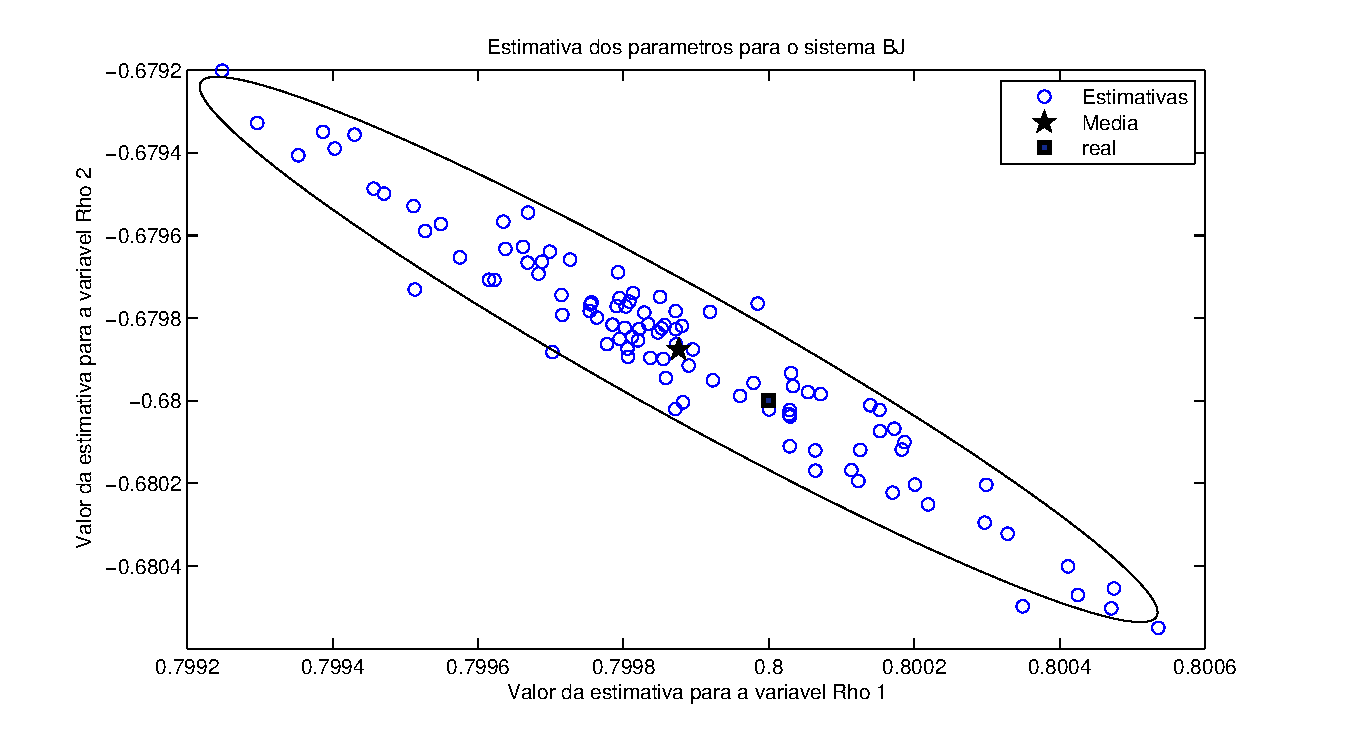
\includegraphics[width=0.95\columnwidth]{figures/vrft_bj_M10_var005.eps}
	\caption{Resultado das 100 estimativas de Monte Carlo dos par�metros $\rho_1$ e $\rho_2$ para o controlador
	apresentado em \eqref{eq:vrft_methos_ex_bj_c}.}
	\label{fig:vrft_bj_M10_var005}
\end{figure}

Os par�metros reais esperados para o controlador (equa��o \eqref{eq:vrft_methos_ex_bj_cd}) e a m�dia de todas
as estimativas (valor representado por uma estrela na Figura (\ref{fig:vrft_bj_M10_var005})) n�o s�o os
mesmos. Em uma situa��o onde o erro de polariza��o das estimativas n�o existe, o aumento de N (n�mero de
amostras) implica que esta diferen�a diminui, tendendo a zero. Em um cen�rio onde h� erro de polariza��o, se 
aumentarmos a vari�ncia do ruido do sistema, ser� observado um aumento desta diferen�a.

Na figura (\ref{fig:vrft_bj_M10_var02}) quadruplicou-se a vari�ncia do ruido inserido no sistema ($\sigma
_\upsilon ^2=0.02$). Observa-se ent�o que o erro de polariza��o existe na estimativa. Como descrito em
\cite{campi_leccini_savaresi2002} quando o m�todo do VRFT � utilizado com ruido nas amostras, a estimativa �
inevitavelmente polarizada. Neste mesmo trabalho � sugerido a utiliza��o de {\it{vari�veis instrumentais}}
(Se��o (\ref{sec:si_par_estim_iv})) para que este erro de polariza��o seja minimizado.

\begin{figure}[htbp] 
	\center 
	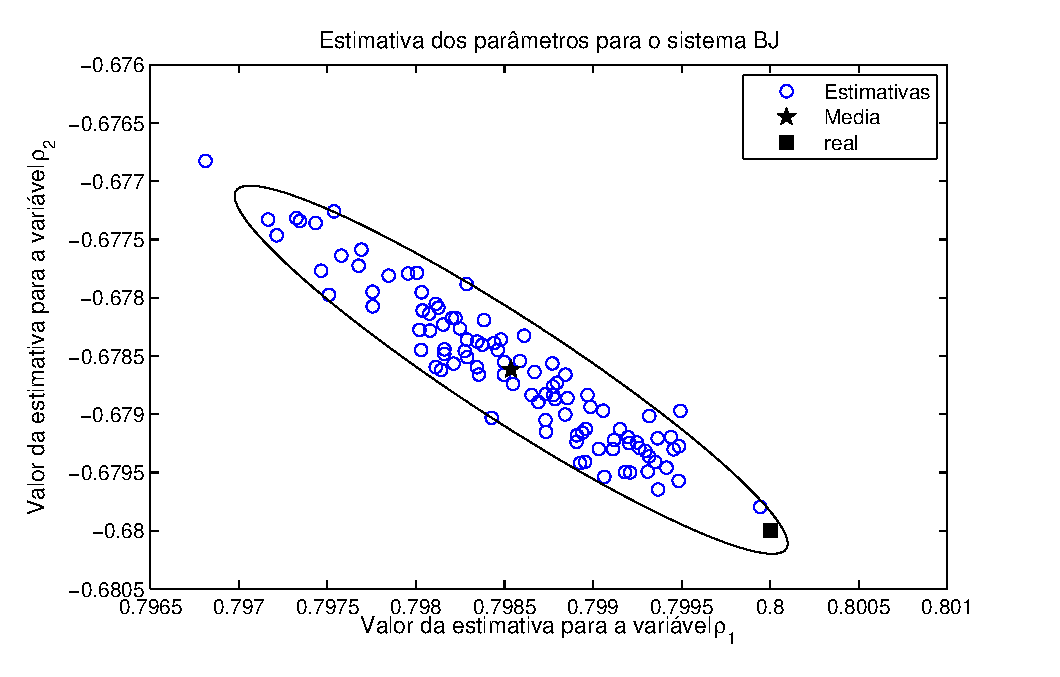
\includegraphics[width=0.95\columnwidth]{figures/vrft_bj_M10_var02.eps}
	\caption{100 estimativas Monte Carlo dos par�metros $\rho_1$ e $\rho_2$ para o controlador apresentado em
	\eqref{eq:vrft_methos_ex_bj_c} com vari�ncia do ruido de 0.02}
	\label{fig:vrft_bj_M10_var02}
\end{figure}

Utilizando o procedimento descrito na se��o (\ref{sec:vrft_framework_noise}) para dados corrompidos por ruido
o resultado obtido, para a mesma vari�ncia de $\sigma_\upsilon ^2=0.02$ do ruido, � apresentado na Figura
(\ref{fig:vrft_bj_M10_var02_iv}).

\begin{figure}[htbp]
	\center
	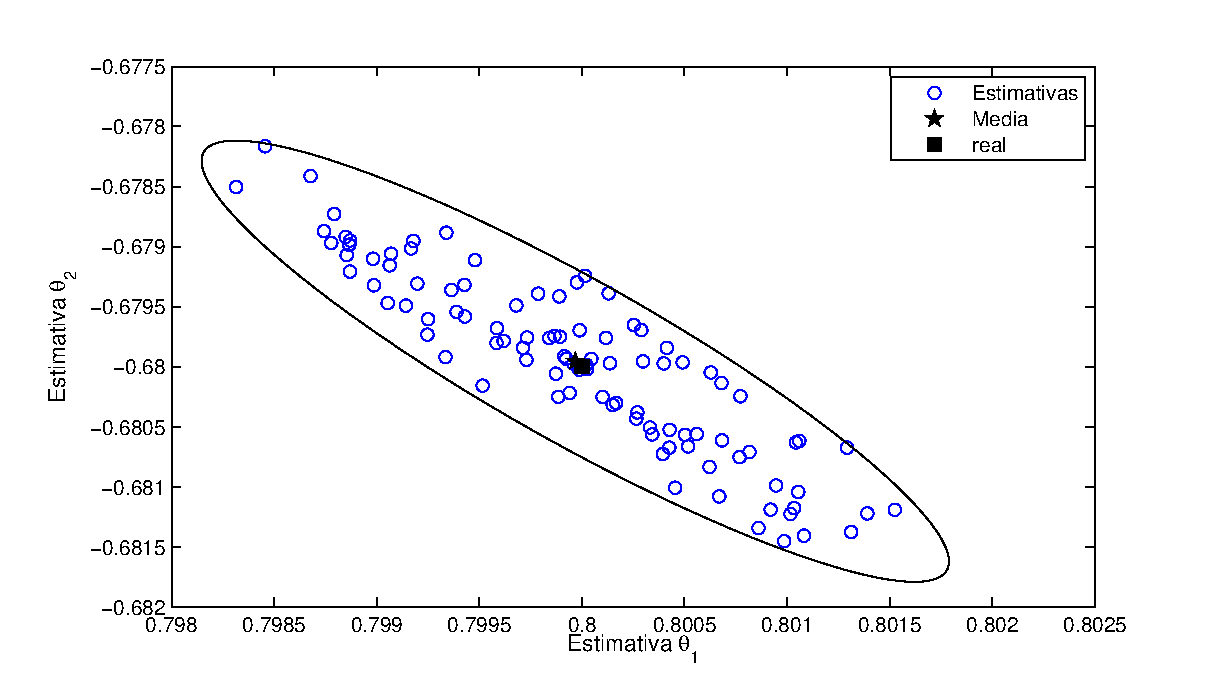
\includegraphics[width=0.95\columnwidth]{figures/vrft_bj_M10_var02_iv.eps}
	\caption{Resultado das 100 estimativas de Monte Carlo dos par�metros $\rho_1$ e $\rho_2$ para o
	controlador apresentado em \eqref{eq:vrft_methos_ex_bj_c} com vari�ncia do
	ruido de 0.02. Utilizando vari�veis instrumentais para estimar os par�metros.}
	\label{fig:vrft_bj_M10_var02_iv}
\end{figure}

Observa-se que o erro de polariza��o foi minimizado e que o resultado obtido possui um custo $J_{VR}^N(\theta)
= 5.1242$ e a vari�ncia dos par�metros estimados foi de $0.5064\times10^{-6}$ para $\rho_1$ e de
$0.5495\times10^{-6}$ para $\rho_2$.

A fim de comparar o m�todo VRFT utilizando e n�o utilizando vari�veis instrumentais s�o apresentados abaixo as
Tabelas (\ref{table:vrft_method_bj}) e (\ref{table:vrft_method_bj_iv}) onde o custo $J_{MR}$ (equa��o
\eqref{eq:vrft_method_cost_func}) e o custo $J_{VR}^N$ (equa��o \eqref{eq:vrft_method_filter_criter_assim})
s�o apresentados para diferentes valores de vari�ncia do ruido para o mesmo sistema BJ.

\begin{table*}[htbp]
\begin{center}
\caption{Valor dos custos $J_{VR}^N$ e $J_{MR}$ al�m da  vari�ncia das
estimativas para diferentes valores de $\sigma _\upsilon ^2$ quando o m�todo
VRFT n�o utiliza vari�veis instrumentais para a estimativa dos par�metros
$\rho$}
\label{table:vrft_method_bj}
\begin{tabular}{cccc}
\hline
        Vari�ncia $\sigma _\upsilon ^2$ & $J_{VR}^N(\theta)$ &
        $J_{MR}(\theta)$ & Vari�ncia estimativas $\rho$   \\
\hline
	    0.06    & 1.7893$\times10^{-2}$ & 8.2367$\times10^{-3}$ & 1.0$\times10^{-5}$\;[0.4754    0.4434] \\
	    0.05    & 1.2515$\times10^{-2}$ & 5.5366$\times10^{-3}$ & 1.0$\times10^{-5}$\;[0.2671    0.3244] \\
        0.04    & 8.1897$\times10^{-3}$ & 3.6071$\times10^{-3}$ & 1.0$\times10^{-5}$\;[0.1534    0.1583] \\
        0.01    & 4.9665$\times10^{-4}$ & 2.4402$\times10^{-4}$ & 1.0$\times10^{-6}$\;[0.0963    0.1035] \\
        0.005   & 1.2515$\times10^{-4}$ & 5.6013$\times10^{-5}$ & 1.0$\times10^{-7}$\;[0.2999    0.3114] \\
        0.001   & 5.0036$\times10^{-6}$ & 3.5734$\times10^{-6}$ & 1.0$\times10^{-8}$\;[0.1301    0.1223] \\
\hline
\end{tabular}
\end{center}
\end{table*} 
   

\begin{table*}[htbp]
\begin{center}
\caption{Valor dos custos $J_{VR}^N$ e $J_{MR}$ al�m da  vari�ncia das
estimativas para diferentes valores de $\sigma _\upsilon ^2$ quando o m�todo
VRFT utiliza vari�veis instrumentais para a estimativa dos par�metros $\rho$}
\label{table:vrft_method_bj_iv}
\begin{tabular}{cccc}
\hline
        Vari�ncia $\sigma _\upsilon ^2$ & $J_{VR}^N(\theta)$ &
        $J_{MR}(\theta)$ & Vari�ncia estimativas $\rho$   \\
\hline
	    0.06    & 45.1719  &  $9.7345\times10^{-5}$ & $1.0\times10^{-5}\;[0.5161    0.5332]$ \\
	    0.05    & 33.2600  &  $2.0457\times10^{-5}$ & $1.0\times10^{-5}\;[0.2481    0.2652]$ \\
        0.04    & 21.2652  &  $1.1665\times10^{-4}$ & $1.0\times10^{-5}\;[0.2040    0.2084]$ \\
        0.01    & 1.2956   &  $8.9695\times10^{-6}$ & $1.0\times10^{-6}\;[0.1246    0.1138]$ \\
        0.005   & 0.3264   &  $7.4764\times10^{-6}$ & $1.0\times10^{-7}\;[0.3063    0.2917]$ \\
        0.001   & 0.0126   &  $5.2443\times10^{-7}$ & $1.0\times10^{-8}\;[0.1059    0.1017]$ \\
\hline
\end{tabular}
\end{center}
\end{table*}

Utilizando vari�veis instrumentais observa-se que o custo $J_{MR}(\theta)$ � significativamente mais baixo
quando comparado com o m�todo onde n�o s�o utilizadas vari�veis instrumentais. Demonstrando assim que o
comportamento desejado do sistema foi atingido com uma melhor aproxima��o.

%===============================================================================
\subsubsection{Controlador PID - sistema ARX}
\label{sec:vrft_examples_pid_arx}
%===============================================================================

Para um sistema {\it{ARX}} onde $G_0(z)$ e $H_0(z)$ podem ser definidos como:

\begin{equation}
G_{ 0 }(z)=\frac { z }{ (z-0.9)(z-0.8) } ,\quad \quad \quad H_{ 0 }(z)=\frac { z^2 }{ (z-0.9)(z-0.8) } 
\nonumber
\end{equation}

Deseja-se que o sistema em malha fechada comporte-se o mais pr�ximo poss�vel do modelo apresentado em:

\begin{equation}
M(z)=\frac { 0.4 }{ z-0.6 }
\label{eq:vrft_methos_ex_arx_M}
\end{equation}

Tem-se assim que o controlador ideal, aquele que ao ser inserido no sistema em
malha fechada apresentado na Figura (\ref{fig:vrft_db_control_loop}) propicia o
comportamento descrito por \eqref{eq:vrft_methos_ex_arx_M} �:

\begin{equation}
C_d(z)=\frac { 0.4(z - 0.9)(z-0.8) }{ z(z-1) }
\label{eq:vrft_methos_ex_arx_cd}
\end{equation}

Observa-se que este controlador pode ser representado como um controlador
{\it{PID}} como em \eqref{eq:vrft_methos_ex_arx_c}. 

\begin{equation}
C(z,\rho )=\frac { \rho _{ 1 }z^2+\rho _{ 2 }z+\rho _{ 3 } }{ z(z-1) } 
\label{eq:vrft_methos_ex_arx_c}
\end{equation}

Na Figura (\ref{fig:vrft_arx_M10_var005}) � apresentado o resultado da estimativa dos par�metros do
controlador quando n�o s�o utilizados vari�veis instrumentais. Obteve-se desta forma um custo
$J_{VR}^N(\theta) = 2.5008\times10^{-5}$ e $J_{MR}(\theta) = 1.7746\times10^{-5}$ al�m de uma vari�ncia para as
estimativas de $1.0\times10^{-7} \; [0.0364\;    0.1261\;    0.0377]$ para $\rho_1$, $\rho_2$ e $\rho_3$
respectivamente.

\begin{figure}[htbp] 
	\center 
	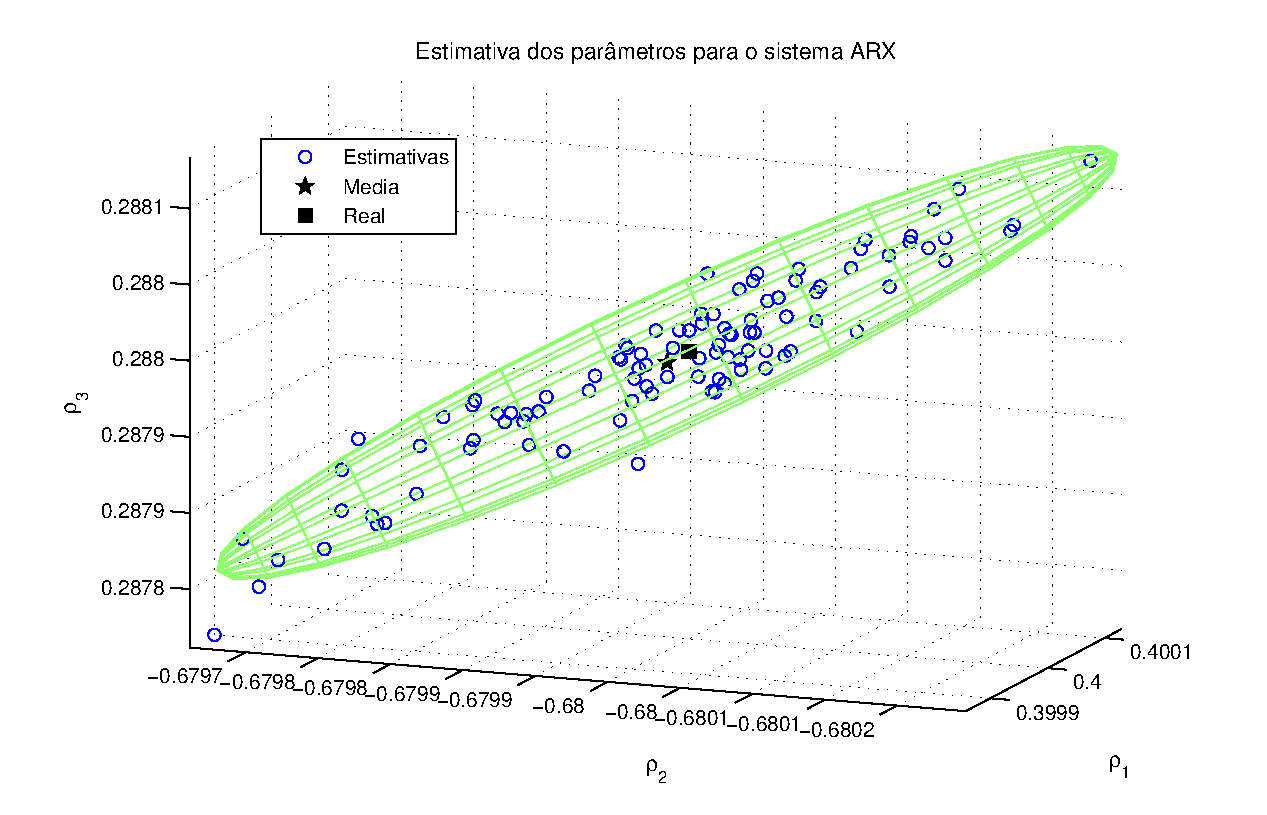
\includegraphics[width=0.95\columnwidth]{figures/vrft_arx_M10_var005_.eps}
	\caption{100 estimativas Monte Carlo dos par�metros $\rho_1$, $\rho_2$ e $\rho_3$ para o controlador
	apresentado em \eqref{eq:vrft_methos_ex_arx_c} com vari�ncia do ruido $\sigma_\upsilon ^2=0.005$}
	\label{fig:vrft_arx_M10_var005}
\end{figure}

Como j� foi observado a utiliza��o de vari�veis instrumentais melhora significativamente o erro de polariza��o existente
nas estimativas. Desta forma as informa��es apresentadas a seguir ser�o feitas utilizando vari�veis instrumentais.
Na figura (\ref{fig:vrft_arx_M10_var05_iv}) � apresentado a estimativa dos par�metros do controlador para um
ruido com vari�ncia $\sigma_\upsilon ^2=0.05$. Observa-se que n�o h� erro de polariza��o nas estimativas. 
O custo para esta, e outas, estimativas � apresentado na Tabela (\ref{table:vrft_method_arx_iv}).

\begin{figure}[htbp] 
	\center 
	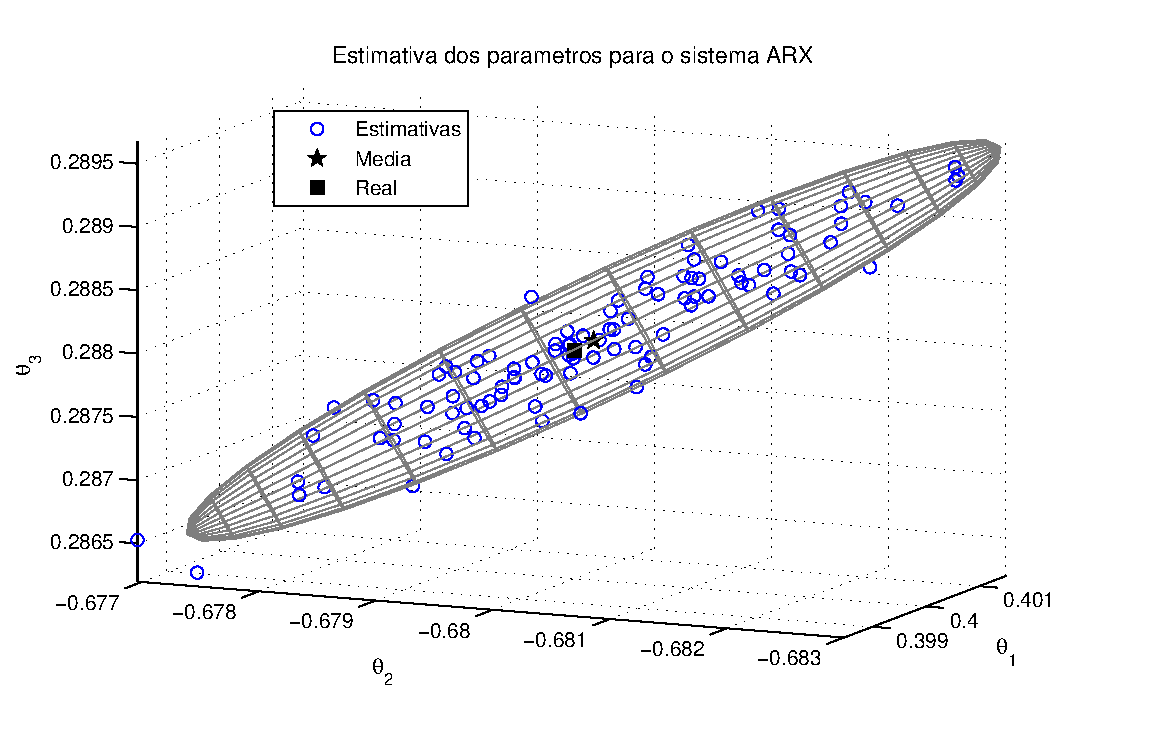
\includegraphics[width=0.95\columnwidth]{figures/vrft_arx_M10_var05_iv.eps}
	\caption{100 estimativas Monte Carlo dos par�metros $\rho_1$, $\rho_2$ e $\rho_3$ para o controlador
	apresentado em \eqref{eq:vrft_methos_ex_arx_c} com vari�ncia do ruido $\sigma_\upsilon ^2=0.05$ utilizando
	vari�veis instrumentais}
	\label{fig:vrft_arx_M10_var05_iv}
\end{figure}


\begin{table*}[htbp]
\begin{center}
\caption{Valor dos custos $J_{VR}^N$ e $J_{MR}$ al�m da  vari�ncia das
estimativas para diferentes valores de $\sigma _\upsilon ^2$ quando o m�todo
VRFT utiliza vari�veis instrumentais para a estimativa dos par�metros $\rho$ do controlador
\eqref{eq:vrft_methos_ex_arx_c}}
\label{table:vrft_method_arx_iv}
\begin{tabular}{cccc}
\hline
        Vari�ncia $\sigma _\upsilon ^2$ & $J_{VR}^N(\theta)$ &
        $J_{MR}(\theta)$ & Vari�ncia estimativas $\rho$   \\
\hline
   0.1     & $10.0743\times10^{-3}$ &  2.2871$\times10^{-3}$ & $1\times10^{-5}\;[0.1253 \; 0.4683 \; 0.1600]$ \\
   0.06    & $ 3.6093\times10^{-3}$ &  1.1279$\times10^{-3}$ & $1\times10^{-5}\;[0.0516 \; 0.1793 \; 0.0575]$ \\
   0.05    & $ 2.5419\times10^{-3}$ &  1.2453$\times10^{-3}$ & $1\times10^{-5}\;[0.0344 \; 0.1237 \; 0.0416]$ \\
   0.04    & $ 1.6013\times10^{-3}$ &  0.5106$\times10^{-3}$ & $1\times10^{-6}\;[0.2195 \; 0.7908 \; 0.2379]$ \\
   0.01    & $10.0077\times10^{-5}$ & 13.7142$\times10^{-5}$ & $1\times10^{-7}\;[0.1552 \; 0.5469 \; 0.1822]$ \\
   0.005   & $ 2.5081\times10^{-5}$ & 10.3482$\times10^{-5}$ & $1\times10^{-7}\;[0.0406 \; 0.1260 \; 0.0375]$ \\
	0.001  & $ 0.1009\times10^{-5}$ &  2.0487$\times10^{-5}$ & $1\times10^{-9}\;[0.1277 \; 0.4035 \;0.1239]$	 \\
\hline
\end{tabular}
\end{center}
\end{table*}

%===============================================================================
\subsubsection{Controlador n�o pertence a classe}
\label{sec:vrft_examples_not_in_class}
%===============================================================================

At� este ponto foram apresentados exemplos de uso do m�todo VRFT quando o controlador que leva o sistema para
o comportamento desejado $M(z)$ faz parte da classe escolhida para a identifica��o. Em outras palavras quando
$C_0(z) \in \mathcal{C(z, \theta)}$. Nesta se��o ser� apresentado um exemplo onde o modelo do controlador escolhido
para o sistema n�o consegue levar este para $M(z)$, ou seja, n�o consegue representar a totalidade das din�micas de
$C_0(z)$.

Considerando o sistema descrito por
\begin{equation}
G_{ 0 }(z)=\frac { 0.2(z-0.7) }{ (z-0.9)(z-0.5) } ,\quad \quad \quad H_{ 0 }(z)=\frac { z }{ z-0.3 } 
\nonumber
\end{equation}

Deseja-se que em malha fechada ele se comporte como em: 

\begin{equation}
M(z)=\frac { 0.16z }{ (z-0.6)^2 }
\label{eq:vrft_methos_ex_pid_not_M}
\end{equation}

Neste caso o controlador ideal � definido por \eqref{eq:vrft_methos_ex_pid_not_cd}

\begin{equation}
C_{ d }(z)=\frac { 0.8z(z-0.9)(z-0.5) }{ (z-1)(z-0.36)(z-0.7) } 
\label{eq:vrft_methos_ex_pid_not_cd}
\end{equation}

Para esta identifica��o optou-se por um controlador do tipo PID como em \eqref{eq:vrft_methos_ex_pid_not_c}
 
\begin{equation}
C(z,\rho )=\frac { \rho _{ 1 }z^2+\rho _{ 2 }z+\rho _{ 3 } }{ z(z-1) } 
\label{eq:vrft_methos_ex_pid_not_c}
\end{equation}

Observa-se que \eqref{eq:vrft_methos_ex_pid_not_c} n�o consegue representar todas as din�micas apresentadas em
\eqref{eq:vrft_methos_ex_pid_not_cd}. Utilizando o procedimento descrito na Se��o
(\ref{sec:vrft_framework_noise}) e o procedimento de experimento repetido, foram feitos 100 experimentos de
Monte Carlo e o resultado obtido para a m�dia das estimativas foi:

\begin{equation}
\rho_L =\left[ 0.8101 \quad -0.1691  \quad -0.3358 \right]
\nonumber
\end{equation}

Onde o �ndice $L$ indica que este resultado foi obtido utilizando-se o filtro $L$.

Repetindo a simula��o, mas agora sem que o procedimento da utiliza��o do filtro $L$ descrito na se��o
(\ref{sec:vrft_framework_noise}), obteve-se o resultado seguinte:

\begin{equation}
\rho =\left[ 0.5846 \quad -0.2108  \quad -0.1525 \right]
\nonumber
\end{equation}

Aplicando-se estes resultados ao controlador apresentado em \eqref{eq:vrft_methos_ex_pid_not_c} e de posse do
comportamento desejado para o sistema em malha fechada ($M(z)$) � poss�vel fazer um comparativo da resposta
ao salto unit�rio para o sistema utilizando os dois controladores obtidos. O resultado � apresentado na Figura
(\ref{fig:vrft_notinclass_step}).

\begin{figure}[htbp] 
	\center 
	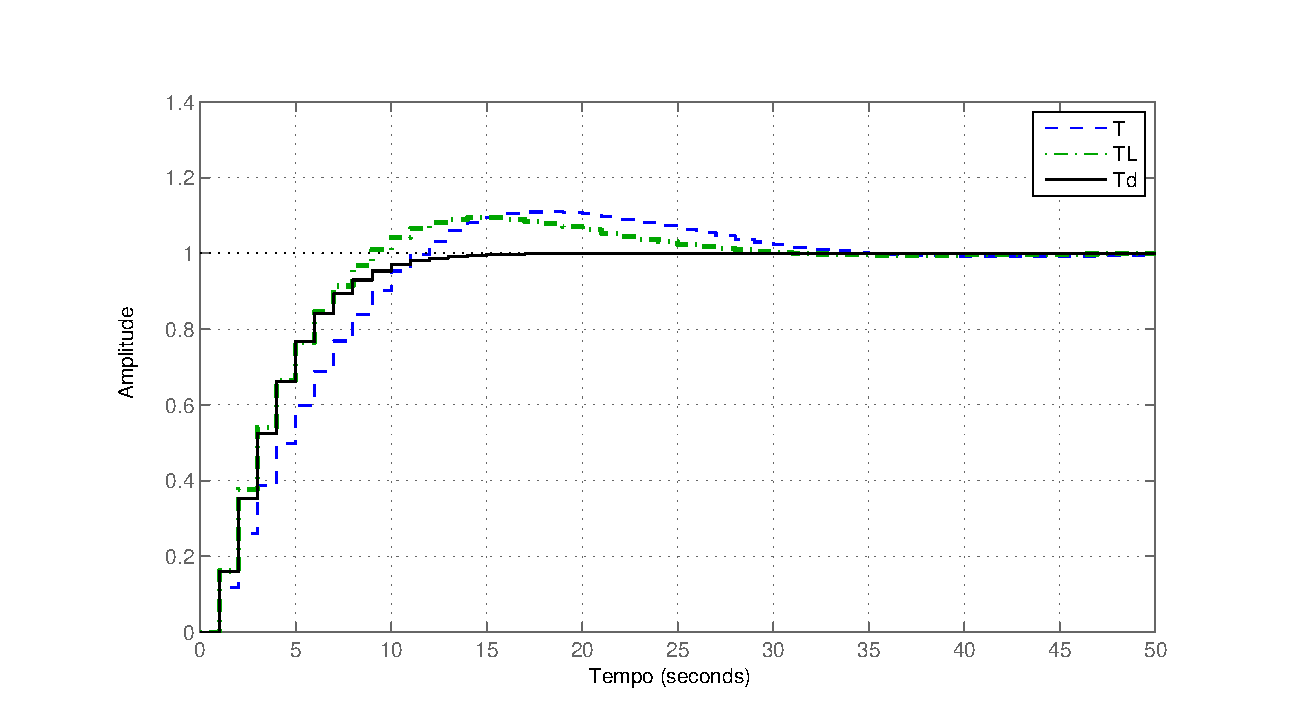
\includegraphics[width=0.95\columnwidth]{figures/vrft_notinclass_step.eps}
	\caption{Comparativo da resposta do sistema a um degrau unit�rio quando o controlador inserido � obtido pelo
	m�todo VRFT utilizando o filtro L e quando n�o se utiliza este artificio. O sistema foi simulado com um
	ruido de vari�ncia $\sigma_\upsilon ^2=0.1$}
	\label{fig:vrft_notinclass_step}
\end{figure}

Observa-se que para o sistema que utiliza o controlador estimado utilizando-se o filtro $L$, a resposta ao
degrau unit�rio tem significativamente menos erro que o sistema utilizando o outro controlador. Ficando este
primeiro muito mais pr�ximo da fun��o $M(z)$ desejada.

Os custos destes dois sistemas � apresentado na Tabela (\ref{table:vrft_method_notinclass}).

\begin{table*}[htbp]
\begin{center}
\caption{Valor dos custos $J_{VR}^N$ e $J_{MR}$ para o sistema controlado por $C(z)$ e $C_L(z)$}
\label{table:vrft_method_notinclass}
\begin{tabular}{ccc}
\hline
        Controlador & $J_{VR}^N(\theta)$ & $J_{MR}(\theta)$ \\
\hline
	$C(z)$   & 0.2877 &  0.1270 \\
	$C_L(z)$ & 0.4481 &  0.0542 \\
\hline
\end{tabular}
\end{center}
\end{table*}

A fim de comparar as duas estimativas, na figura (\ref{fig:vrft_notinclass_bode}) � apresentado o diagrama de
Bode dos controladores obtidos (utilizando a m�dia das estimativas obtidas).

\begin{figure}[htbp] 
	\center 
	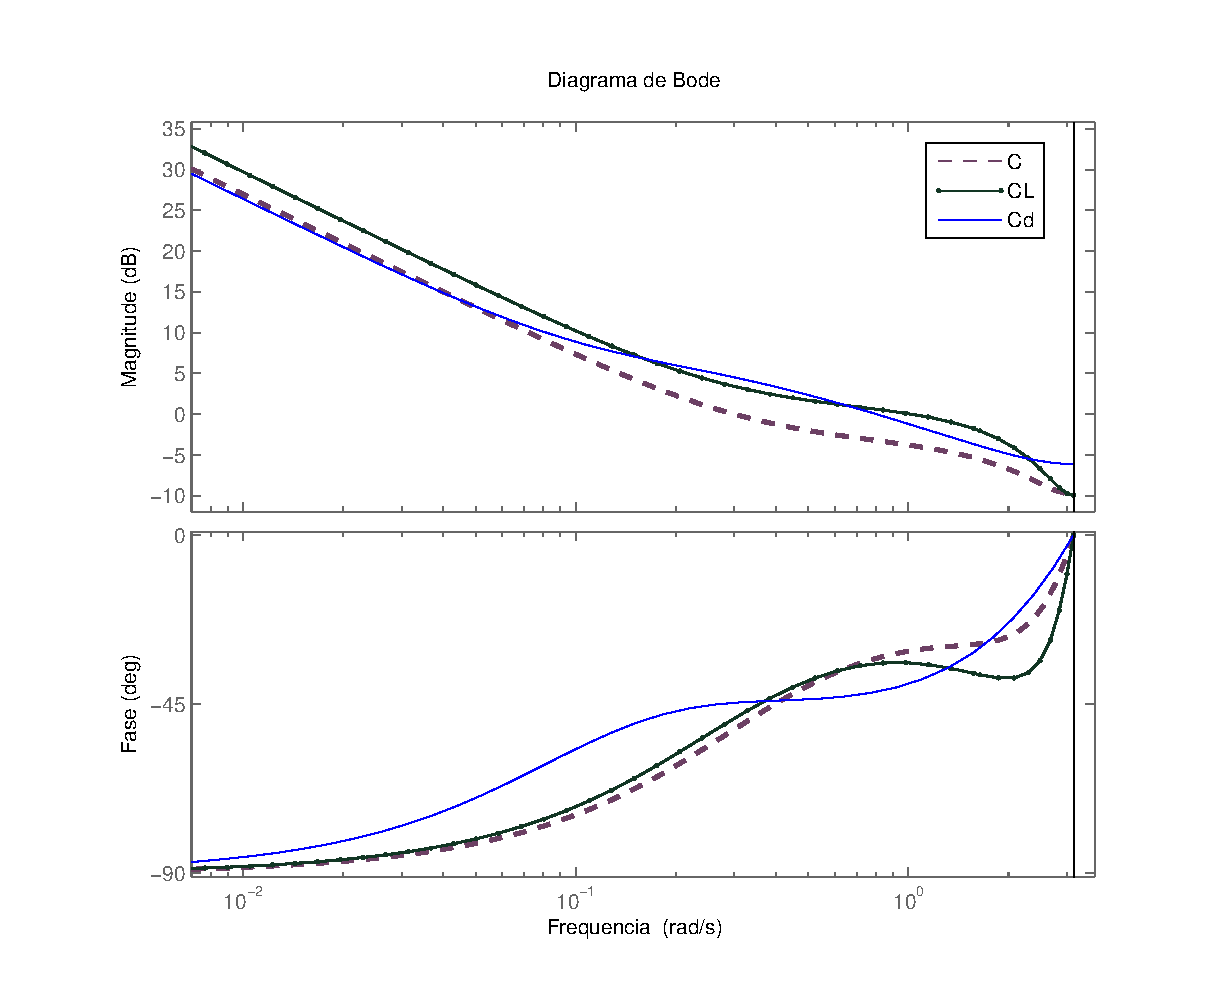
\includegraphics[width=0.99\columnwidth]{figures/vrft_notinclass_bode.eps}
	\caption{Diagrama de Bode para as fun��es de transfer�ncia dos controladores estimados utilizando VRFT com e
	sem o artificio do filtro L e vari�veis instrumentais}
	\label{fig:vrft_notinclass_bode}
\end{figure}


% ===============================================================================
\section{Identifica��o de sistemas n�o lineares utilizando refer�ncia virtual}
\label{sec:vrft_nonlinear}
%===============================================================================

Como visto na se��o \ref{sec:vrft_vrft}, o m�todo VRFT tem um grande apelo, e produz resultados
significativamente satisfat�rios para diversos modelos lineares. 

Nesta se��o o objetivo � demonstrar como este m�todo de comporta com sistemas n�o lineares. Duas
n�o linearidades ser�o apresentadas: est�ticas, para isso ser� utilizado o modelo de Wiener (apresentado na
se��o \ref{sec:nl_models_wiener_hammerstein}) e n�o linearidades din�micas, a classe de modelos escolhido
foram modelos NARMAX racionais (apresentados na se��o \ref{sec:nl_models_narmax_rat}).

A fun��o custo que pretende-se minimizar pode ser expressa como:

\begin{equation}
J(\theta)=\left \| y_{\theta}-M \tilde{r} \right \|^2
\label{eq:vrft_nl_j}
\end{equation} 

Onde $y_{\theta}=G\left [ C_{\theta}\left [ \tilde{r} -D y_{\theta} \right ] \right ]$ e $D$ � o atraso da
planta.

Desta forma o que se observa � que o custo a ser minimizado � dependente da planta que a-priori �
desconhecida. Ent�o � sugerido a minimiza��o de outra fun��o custo que possui a o mesmo minimo que
\eqref{eq:vrft_nl_j}: \cite{campi_savaresi2006}

\begin{equation}
J_{VRFT}(\theta)=\left \| F\left [ C_{\theta}[\tilde{e}] - F[\tilde{u}] \right ] \right \|^2
\label{eq:vrft_nl_jvrft}
\end{equation} 

Onde $F: \mathbb{R}^N\to \mathbb{R}^N$ � um filtro de que deve ser escolhido.

Em \cite{campi_savaresi2006} indica-se a utiliza��o do filtro:

\begin{equation}
F=(I-MD) \left ( \frac{\partial G\left [ u \right ]}{\partial u}|_{\tilde{u}} \right ) 
\label{eq:vrft_nl_filter}
\end{equation} 

Onde $ \frac{\partial G\left [ u \right ]}{\partial u}$ deve ser calculado a partir dos dados coletados.
Imprecis�es nesta estimativa apenas indicam que a segunda derivada de $J_{VRFT}$ n�o ir� precisamente
ter o mesmo m�nimo que $J$. \cite{campi_savaresi2006}

Devido ao custo e dificuldade de se obter $ \frac{\partial G\left [ u \right ]}{\partial u}$ e com o intuito
de utilizar o algoritmo de identifica��o de sistemas racionais apresentados na se��o
\ref{sec:nl_si_algorithms_rationals} optou-se em utilizar sistemas n�o lineares que pudessem ser aproximados
por equa��es n�o lineares racionais ou polinomiais. E desta forma utilizar a metodologia VRFT para gerar os
sinais $\bar{r}(t)$ e $e(t)$, e com isso alimentar o algoritmo de identifica��o de modelos racionais.

Como j� foi discutido, utilizando o m�todo VRFT, pode-se obter os sinais de alimenta��o do controlador, e de
posse do sinal de sa�da deste � poss�vel identificar o controlador que melhor atinge o almejado comportamento
da planta em malha fechada, descrito por $M(z)$.

Desta forma, o que foi alterado do m�todo cl�ssico do VRFT foi a utiliza��o do algoritmo de identifica��o de
modelos racionais, alimentando-o com o sinal de refer�ncia virtual $\bar{r}(t)$ e a sa�da $u(t)$.

A seguir ser�o apresentados alguns exemplos do uso deste procedimento e os resultados obtidos. Os exemplos
ser�o divididos em dois grupos principais: onde existe uma n�o linearidade est�tica na planta, e onde a n�o
linearidade � din�mica.

%===============================================================================
\subsection{N�o linearidades est�ticas}
\label{sec:vrft_nl_wiener}
%===============================================================================

Como n�o linearidade est�tica escolheu-se a classe de modelos de Wiener. Na Figura \ref{fig:vrft_nl_wiener} �
apresentado o diagrama de blocos do sistema, sendo $\Phi$ e $\Phi^{-1}$ os blocos n�o lineares da planta e do
controlador respectivamente.

\begin{figure}[htbp]
\center
% Generated with LaTeXDraw 2.0.8
% Sat May 26 23:30:48 BRT 2012
% \usepackage[usenames,dvipsnames]{pstricks}
% \usepackage{epsfig}
% \usepackage{pst-grad} % For gradients
% \usepackage{pst-plot} % For axes
\scalebox{1} % Change this value to rescale the drawing.
{
\begin{pspicture}(0,-1.32)(11.62,1.3)
\psline[linewidth=0.04cm,arrowsize=0.05291667cm 2.0,arrowlength=1.4,arrowinset=0.4]{->}(0.0,0.3)(0.8,0.3)
\pscircle[linewidth=0.04,dimen=outer](1.0,0.3){0.2}
\psline[linewidth=0.04cm,arrowsize=0.05291667cm 2.0,arrowlength=1.4,arrowinset=0.4]{->}(1.2,0.3)(2.0,0.3)
\psframe[linewidth=0.04,dimen=outer](3.2,0.7)(2.0,-0.1)
\psline[linewidth=0.04cm,arrowsize=0.05291667cm 2.0,arrowlength=1.4,arrowinset=0.4]{->}(3.2,0.3)(4.2,0.3)
\psframe[linewidth=0.04,dimen=outer](5.4,0.7)(4.2,-0.1)
\psframe[linewidth=0.04,dimen=outer](8.0,0.7)(6.8,-0.1)
\psline[linewidth=0.04cm,arrowsize=0.05291667cm 2.0,arrowlength=1.4,arrowinset=0.4]{->}(8.0,0.3)(9.0,0.3)
\psframe[linewidth=0.04,dimen=outer](10.2,0.7)(9.0,-0.1)
\psline[linewidth=0.04cm,arrowsize=0.05291667cm 2.0,arrowlength=1.4,arrowinset=0.4]{->}(5.4,0.3)(6.8,0.3)
\psline[linewidth=0.04cm,arrowsize=0.05291667cm 2.0,arrowlength=1.4,arrowinset=0.4]{->}(10.2,0.3)(11.6,0.3)
\psline[linewidth=0.04cm,arrowsize=0.05291667cm 2.0,arrowlength=1.4,arrowinset=0.4]{<-}(1.0,0.1)(1.0,-1.3)
\psline[linewidth=0.04cm](1.0,-1.3)(10.8,-1.3)
\psline[linewidth=0.04cm](10.8,-1.3)(10.8,0.3)
\usefont{T1}{ppl}{m}{n}
\rput(0.45828125,0.61){r(t)}
\usefont{T1}{ppl}{m}{n}
\rput(1.5445312,0.61){$\epsilon (t)$}
\usefont{T1}{ppl}{m}{n}
\rput(3.699375,0.61){v(t)}
\usefont{T1}{ppl}{m}{n}
\rput(6.089375,0.61){u(t)}
\usefont{T1}{ppl}{m}{n}
\rput(8.464531,0.61){$\omega(t)$}
\usefont{T1}{ppl}{m}{n}
\rput(10.899375,0.61){y(t)}
\psline[linewidth=0.04cm](1.2,0.1)(1.4,0.1)
\psframe[linewidth=0.04,linestyle=dashed,dash=0.16cm 0.16cm,dimen=outer](5.6,1.3)(1.8,-0.3)
\psframe[linewidth=0.04,linestyle=dashed,dash=0.16cm 0.16cm,dimen=outer](10.4,1.3)(6.6,-0.3)
\usefont{T1}{ppl}{m}{n}
\rput(3.5345314,-0.59){C(z)}
\usefont{T1}{ppl}{m}{n}
\rput(8.544531,-0.59){G(z)}
\usefont{T1}{ppl}{m}{n}
\rput(2.5945313,0.29){$\vartheta(t)$}
\usefont{T1}{ppl}{m}{n}
\rput(9.594531,0.31){$\Phi(t)$}
\usefont{T1}{ppl}{m}{n}
\rput(4.7945313,0.31){C'(z)}
\usefont{T1}{ppl}{m}{n}
\rput(7.4045315,0.31){G'(z)}
\usefont{T1}{ppl}{m}{n}
\rput(8.438125,1.01){Wiener}
\usefont{T1}{ppl}{m}{n}
\rput(3.7610939,1.01){Hammerstein}
\end{pspicture} 
}
\caption{Diagrama de blocos para um sistema n�o linear do tipo Wiener}
\label{fig:vrft_nl_wiener}
\end{figure}

Para este exemplo ser�o utilizadas as seguintes defini��es para o sistema:

\begin{equation}
G'(z)=\frac{0.5}{z-0.9}
\label{eq:vrft_nl_wiener_g}
\end{equation} 

$G'(z)$ � a parte linear da planta do sistema. O comportamento do sistema em malha fechada esperado foi
definido como em $M(z)$:

\begin{equation}
M(z)=\frac{0.4}{z-0.6}
\label{eq:vrft_nl_wiener_m}
\end{equation}  

A n�o linearidade presente na planta do sistema foi escolhida como sendo um polin�mio de terceira ordem
descrito como abaixo:

\begin{equation}
\Phi(\omega)=y(t)=1.5\omega(t)+0.2\omega^3(t)
\label{eq:vrft_nl_wiener_phi}
\end{equation}  

Espera-se ent�o que por $M(z)$ ser linear, que o controlador tenha um bloco que seja o inverso de $\Phi$, para
que a n�o linearidade possa ser cancelada completamente.

Atingir uma express�o anal�tica que descreva $\Phi^{-1}$ n�o � uma tarefa simples. Optou-se ent�o por
aproximar esta fun��o por outro polin�mio de ordem 4, definido por $\vartheta (t)$:

\begin{equation}
\vartheta (\epsilon(t))= v(t) = a_1\epsilon (t) + a_2 \epsilon ^2(t) +a_3 \epsilon ^3(t) +a_4 \epsilon ^4(t)
\label{eq:vrft_nl_wiener_phi_inv}
\end{equation}  

Desconsiderando a parte n�o linear presente na planta, � simples de observar que o controlador �timo que
levaria a planta em malha fechada a ter o comportamento descrito por $M(z)$ �:

\begin{equation}
C_d(z)= \frac{0.8z-0.72}{z-1}
\label{eq:vrft_nl_wiener_cd}
\end{equation}  

O controlador $C_d(z)$ possui uma integrador em sua estrutura. Para evitar problemas de seguimento de
refer�ncia optou-se por n�o identificar esta parte do controlador. Mantendo o denominador como um integrador
e identificando apenas o numerador. Juntamente com a identifica��o do controlador da por��o linear $C_d(z)$ �
necess�rio identificar o polin�mio da equa��o \eqref{eq:vrft_nl_wiener_phi_inv}.

Fazendo-se as substitui��es matem�ticas necess�rias, chega-se a express�o do sinal de sa�da do controlador que
se quer identificar:

\begin{equation}
u(t)=\begin{bmatrix}
\theta_1 & \theta_2 & \theta_3 & \theta_4 & \theta_5 & \theta_6 & \theta_7 & \theta_8
\end{bmatrix}
\begin{bmatrix}
\epsilon (t)\\ 
\epsilon ^2(t)\\ 
\epsilon^3(t)\\ 
\epsilon^4(t)\\ 
\epsilon(t-1)\\ 
\epsilon^2(t-1)\\ 
\epsilon^3(t-1)\\ 
\epsilon^4(t-1)
\end{bmatrix}
\label{eq:vrft_nl_wiener_u}
\end{equation}  

Foram feitos 100 experimentos de Monte Carlo e a m�dia das estimativas obtidas foi de:

\begin{equation}
\text{m�dia }\;\theta =\begin{bmatrix}
0.4471 \\ 0.0020 \\ -6.5105\times10^{-4} \\ -1.5959\times10^{-5} \\ -0.4043 \\ -0.0016 \\ 6.1194\times10^{-4}
\\ 1.4562\times10^{-5}
\end{bmatrix}^T
\nonumber
\end{equation}

Com um desvio padr�o de:

\begin{equation}
\text{m�dia }\;\theta = 1\times10^{-3}\begin{bmatrix}
0.2430 \\ 0.0246 \\ 0.0015 \\ 0.0001 \\ 0.2613 \\ 0.0259 \\ 0.0016 \\ 0.0001
\end{bmatrix}^T
\nonumber
\end{equation}

O custo entre os sinais de sa�da do sistema obtido e o sistema esperado $M(z)$ foi de  $J_{MR}(\theta)=
0.3820$ e o custo dos sinais de sa�da do controlador esperado e obtido foi de $J_{VR}=1.0119$.

Como a estimativa de $\vartheta (\epsilon(t))$ � apenas uma aproxima��o do que espera-se ser a inversa de
$\Phi(\omega(t))$, a classe de modelos escolhida para o controlador n�o consegue representar a totalidade do
controlador ideal. Desta forma � esperado que a identifica��o n�o consiga atingir a totalidade da fun��o
$M(z)$ inicialmente escolhido. Para as estimativas foram utilizados sinais PRBS de 127 pontos para a
excita��o da planta.

Na Figura (\ref{fig:vrft_nl_wiener_step}) � apresentado um comparativo entre o sinal de sa�da do sistema
$M(z)$ quando submetido a um degrau unit�rio e o sinal do sistema real quando o controlador identificado �
aplicado sobre a planta em malha fechada.

\begin{figure}[htbp] 
	\center 
	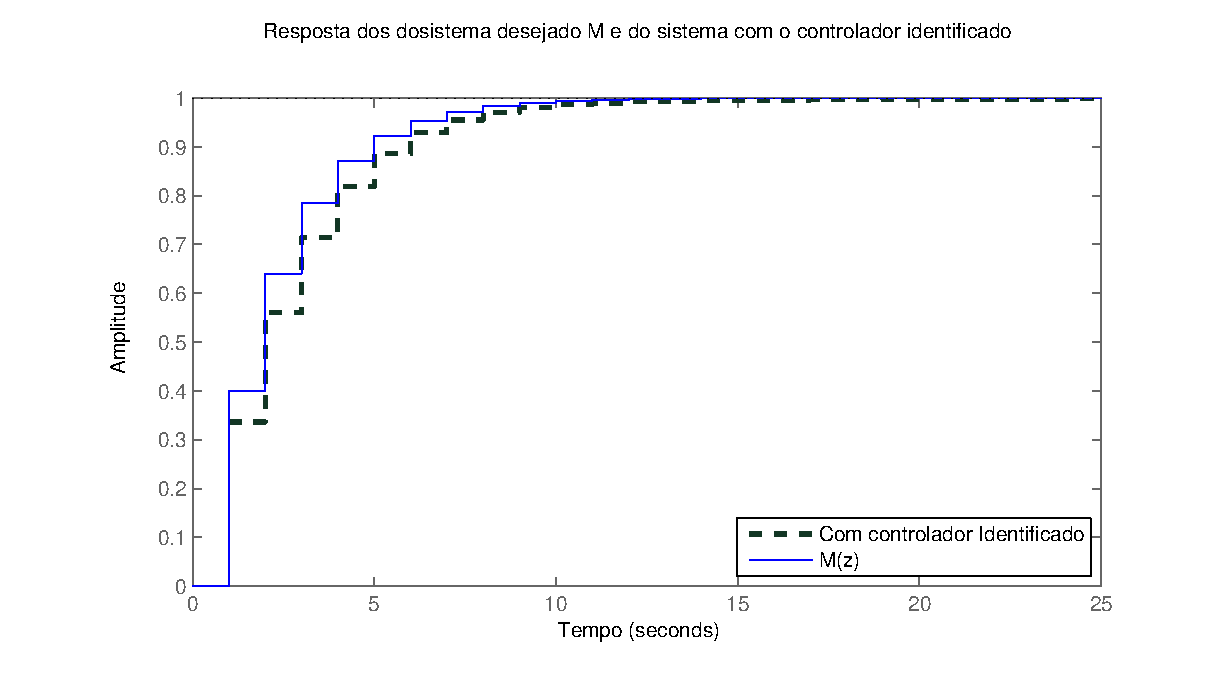
\includegraphics[width=0.95\columnwidth]{figures/vrft_nl_wiener_step.eps}
	\caption{resposta dos sistemas: desejado e obtido a um degrau unit�rio}
	\label{fig:vrft_nl_wiener_step}
\end{figure}

Na Figura (\ref{fig:vrft_nl_wiener_vw_step}) � apresentado o comportamento dos sinais de sa�da e entrada das
n�o linearidades $\Phi^{-1}(e(t))$ e $\Phi(\omega(t))$ respectivamente.

\begin{figure}[htbp] 
	\center 
	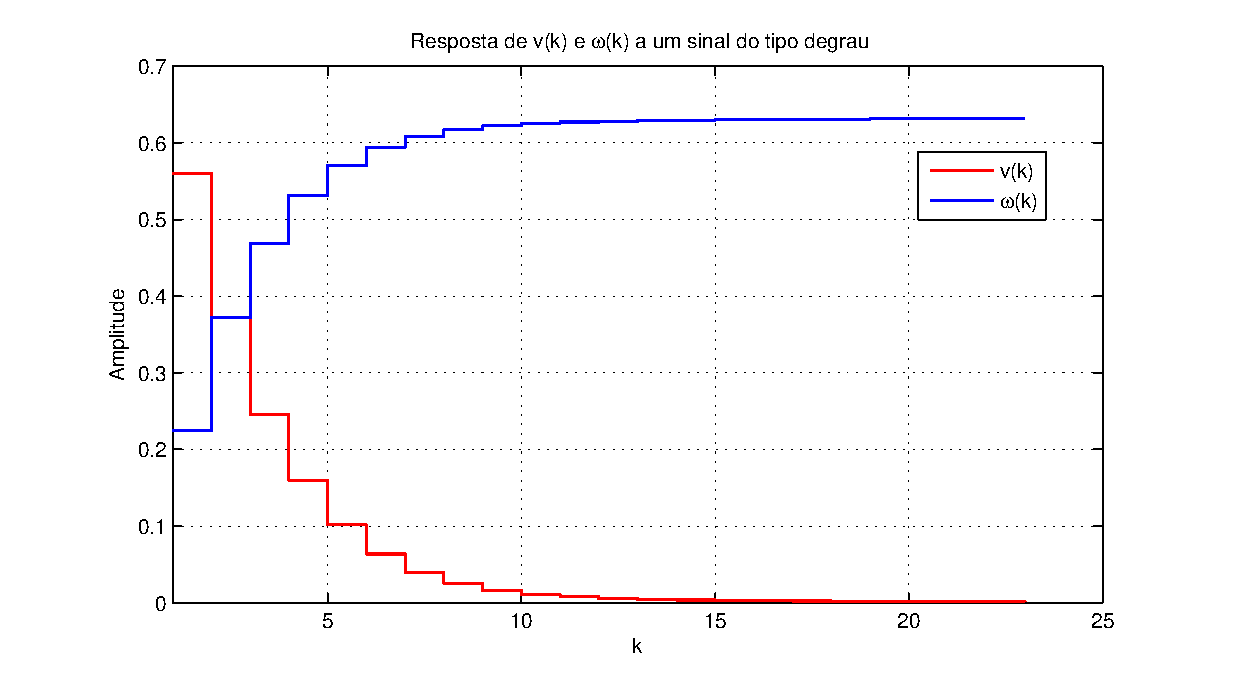
\includegraphics[width=0.95\columnwidth]{figures/vrft_nl_wiener_vw_step.eps}
	\caption{sinais $v(t)$ e $\omega(t)$ quando o sistema � alimentado por um degrau unit�rio}
	\label{fig:vrft_nl_wiener_vw_step}
\end{figure}

A rela��o entre os sinais $v(t)$ e $\omega(t)$ � apresentado na Figura (\ref{fig:vrft_nl_wiener_vw}).
Observa-se que a rela��o destes sinais � praticamente linear, garantido que a aproxima��o de $\Phi^{-1}$ foi
satisfat�ria para representar a inversa do sinal $\Phi$.

\begin{figure}[htbp] 
	\center 
	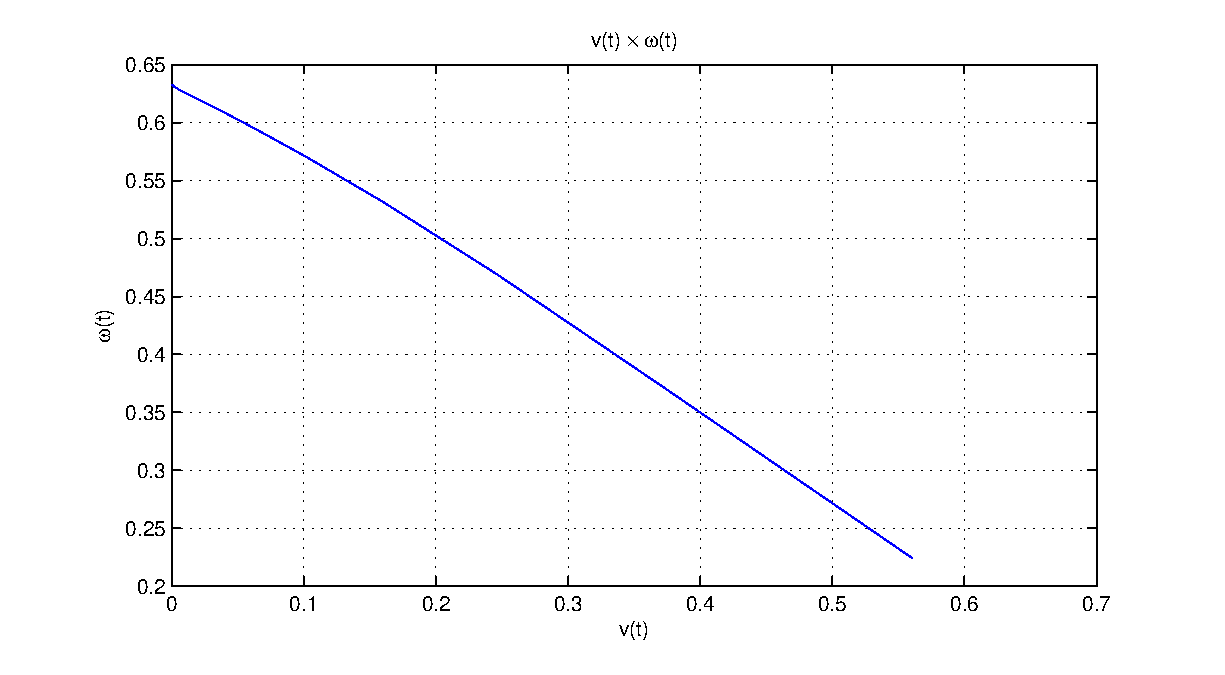
\includegraphics[width=0.95\columnwidth]{figures/vrft_nl_wiener_vw.eps}
	\caption{rela��o entre os sinais $v(t)$ e $\omega(t)$ quando o sistema � alimentado por um degrau unit�rio}
	\label{fig:vrft_nl_wiener_vw}
\end{figure}

%===============================================================================
\subsection{N�o linearidades din�micas}
\label{sec:vrft_nl_dinamic}
%===============================================================================
Nesta se��o ser�o apresentados alguns exemplos do algoritmo apresentado na Se��o
\ref{sec:nl_si_algorithms_rationals} em conjunto com o principio b�sico do m�todo VRFT para a obten��o dos
sinais $r(t)$ e $e(t)$, al�m do sinal escolhido $u(t)$ utilizado para excitar a planta e o pr�prio sinal de
sa�da da planta $y(t)$.

\TODO: escrever algo mais aqui !!!!!!

%===============================================================================
\subsubsection{Controlador sendo representado pelo modelo}
\label{sec:vrft_nl_dinamic_c_match}
%===============================================================================

Considere a planta descrita por:

\begin{equation}
y(t)=\frac{0.1u(t-1)y(t-1)+u(t-1)}{1+0.25y^2(t-2)}
\label{eq:vrft_nl_dinamic_ex1_y}
\end{equation}

Deseja-se que em malha fechada seu comportamento seja como em:

\begin{equation}
M(z)=\frac{Y(z)}{R(z)}=\frac{0.4}{z-0.6}
\label{eq:vrft_nl_dinamic_ex1_mz}
\end{equation}

A equa��o de $M(z)$ pode ser reescrita em fun��o do tempo como em:

\begin{equation}
y(t)=0.4r(t-1)+0.6y(t-1)
\label{eq:vrft_nl_dinamic_ex1_mt}
\end{equation}

Ao igualarmos a equa��o \eqref{eq:vrft_nl_dinamic_ex1_y} com \eqref{eq:vrft_nl_dinamic_ex1_mt} e isolando o
sinal $u(t)$ temos a equa��o que descreve o comportamento do controlador que levar� a planta a ter o
comportamento descrito por $M(z)$ em malha fechada. Obt�m-se desta forma um controlador ideal como em:

\begin{equation}
u(t)=\frac{0.4r(t)+0.6y(t)+0.1y^2(t-2)r(t-1)+0.15y(t)y^2(t-1)}{1+0.5y(t)}
\label{eq:vrft_nl_dinamic_ex1_cd}
\end{equation}

Escolhendo um conjunto de modelos que consegue representar o controlador �timo:

\begin{equation}
u(t)=\frac{\theta_1 r(t)+ \theta_2 y(t)+ \theta_3 y^2(t-2)r(t-1)+ \theta_4 y(t)y^2(t-1)}{1+ \theta_5 y(t)}
\label{eq:vrft_nl_dinamic_ex1_c}
\end{equation}

Utilizando um sinal PRBS de tamanho 254 e o m�todo do VRFT para gerar os sinais $r(t)$ e $e(t)$. 
Adicionando-se um ruido de vari�ncia $\sigma^2 = 0.005$, a m�dia da estimativa para 100 experimentos de
Monte Carlo foi de:


\begin{equation}
\text{m�dia de }\theta=\begin{bmatrix}
0.4000 & 0.5999 & 0.1001 & 0.1501 & 0.5000
\end{bmatrix}
\nonumber
\end{equation}

\begin{equation}
\text{Desvio padr�o de }\theta=1.0\times 10^{-3}\begin{bmatrix}
0.2231 & 0.6866 & 0.2411 & 0.6817 & 0.3019
\end{bmatrix}
\nonumber
\end{equation}

\begin{equation}
\text{Covari�ncia }\theta=1.0\times 10^{-6}\begin{bmatrix}
 0.0498 &  0.0585 & -0.0353 & -0.0362 & -0.0018 \\
 0.0585 &  0.4714 & -0.0449 & -0.3690 &  0.0057 \\
-0.0353 & -0.0449 &  0.0581 &  0.0745 & -0.0040 \\
-0.0362 & -0.3690 &  0.0745 &  0.4647 & -0.0070 \\
-0.0018 &  0.0057 & -0.0040 & -0.0070 &  0.0911
\end{bmatrix}
\nonumber
\end{equation}

Simulando o sistema obtido com o controlador estimado e o sistema em malha fechada desejado, o erro observado
� apresentado na figura \ref{fig:vrft_nl_dynamic_step_erro}.

\begin{figure}[htbp] 
	\center 
	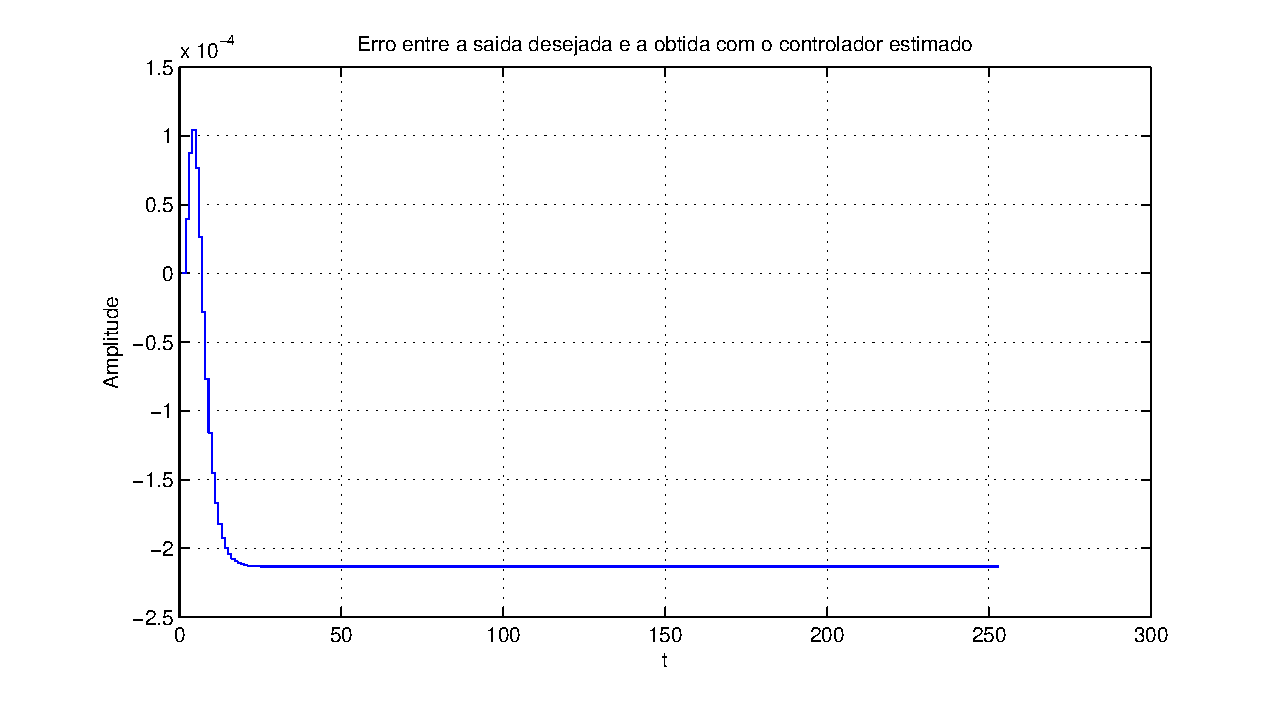
\includegraphics[width=0.95\columnwidth]{figures/vrft_nl_dynamic_erro_step.eps}
	\caption{Erro entre o a resposta esperada e obtida para uma entrada do tipo degrau unit�rio}
	\label{fig:vrft_nl_dynamic_step_erro}
\end{figure}

E a fim de ilustrar as estimativas obtidas pelo m�todo, na Figura \ref{fig:vrft_nl_dynamic_t1_t2} s�o
apresentados as estimativas para os 100 experimentos realizados, al�m da elipse de confian�a de $\chi^2=95\%$
para os parametros $\theta_1$ e $\theta_2$.

\begin{figure}[htbp] 
	\center 
	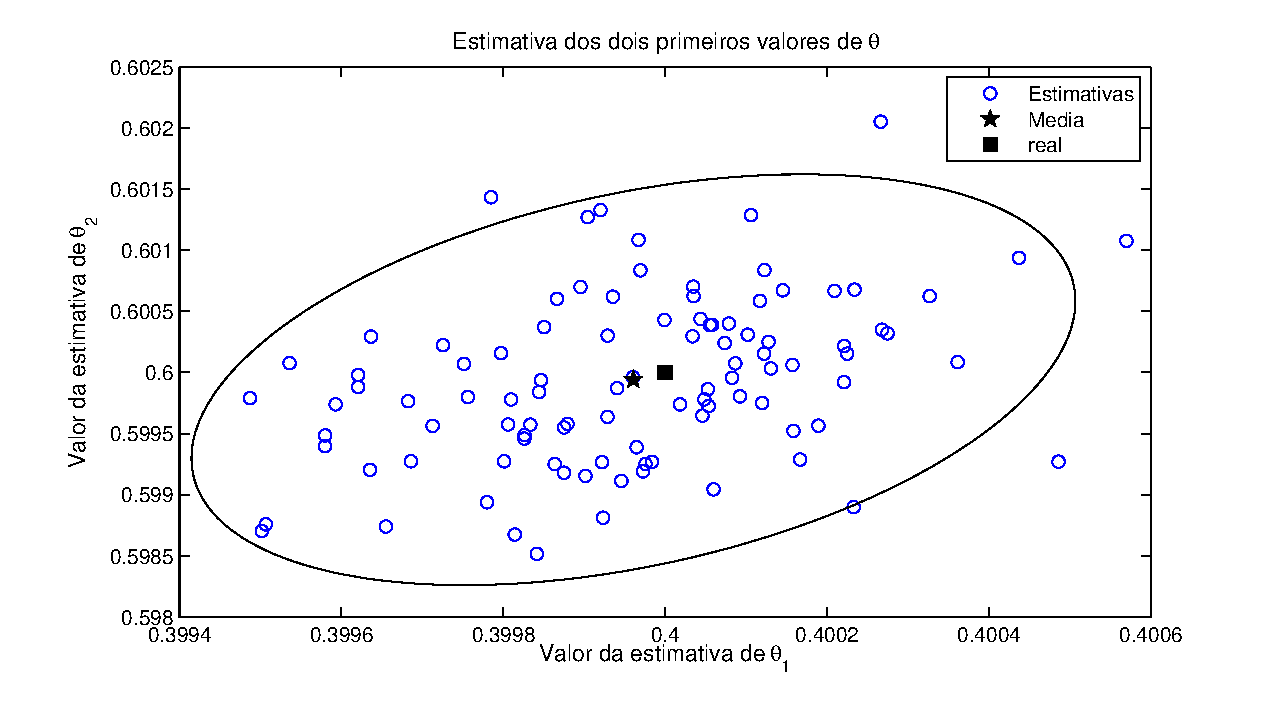
\includegraphics[width=0.95\columnwidth]{figures/vrft_nl_dynamic_t1_t2.eps}
	\caption{100 esperimentos de Monte Carlo das vari�veis $\theta_1$ e $\theta_2$}
	\label{fig:vrft_nl_dynamic_t1_t2}
\end{figure}

O custo $J_{VRFT}=2.7291\times10{-8}$ foi obtido utilizando-se os sinais de sa�da do controlador obtido e
esperado. J� o custo entre os sinais de sa�da do sistema em malha fechada estimado e desejado foi de
$J_{MR}=0.0033$.


\cite{lecchini_campi_savaresi_2dof}
\cite{Guardabassi}



%ruido de 0.01
%
%mtheta =
%
%    0.4000    0.5997    0.1000    0.1503    0.5007
%
%
%vartheta =
%
%   1.0e-04 *
%
%    0.0609    0.6407    0.0593    0.4256    0.0970
%
%
%stdtheta =
%
%    0.0025    0.0080    0.0024    0.0065    0.0031
%
%
%covtheta =
%
%   1.0e-04 *
%
%    0.0609    0.1062   -0.0435   -0.0642   -0.0062
%    0.1062    0.6407   -0.0792   -0.4292    0.0071
%   -0.0435   -0.0792    0.0593    0.0902   -0.0097
%   -0.0642   -0.4292    0.0902    0.4256   -0.0194
%   -0.0062    0.0071   -0.0097   -0.0194    0.0970
%
%
%Jvr_nl =
%
%   1.9177e-06
%
%
%Jmr_nl =
%
%    0.0148
%
%===============================================================================
\subsubsection{Controlador sendo representado pelo modelo 2}
\label{sec:vrft_nl_dinamic_c_match2}
%===============================================================================

%===============================================================================
\subsubsection{Controlador n�o sendo representado pelo modelo}
\label{sec:vrft_nl_dinamic_c_not_match}
%===============================================================================








































%===============================================================================
\section{Considera��es Finais}
\label{sec:vrft_conclusions}
%===============================================================================


%===============================================================================

